% =============================================================================
% MLSys·im ISCA 2026 Tutorial — Parts 0–4 (Morning Session)
% =============================================================================
% Compile standalone: xelatex tutorial_part1.tex   (or pdflatex)
% Requires: metropolis beamer theme (texlive-full or tlmgr install metropolis)
% =============================================================================
\documentclass[aspectratio=169, 12pt]{beamer}
\usetheme{metropolis}

% --- Brand colors (matching mlsys theme) ---
\definecolor{crimson}{HTML}{A51C30}
\definecolor{darkcrimson}{HTML}{7A1020}
\definecolor{computeblue}{HTML}{CFE2F3}
\definecolor{computestroke}{HTML}{4A90C4}
\definecolor{datagreen}{HTML}{D4EDDA}
\definecolor{datastroke}{HTML}{3D9E5A}
\definecolor{routingorange}{HTML}{FDEBD0}
\definecolor{routingstroke}{HTML}{C87B2A}
\definecolor{errorfill}{HTML}{F9D6D5}
\definecolor{errorstroke}{HTML}{CC4444}
\definecolor{darktext}{HTML}{1A1A2E}
\definecolor{midgray}{HTML}{555555}

% --- Apply to Beamer elements ---
\setbeamercolor{frametitle}{bg=crimson, fg=white}
\setbeamercolor{progress bar}{fg=crimson}
\setbeamercolor{alerted text}{fg=crimson}
\setbeamercolor{palette primary}{bg=crimson, fg=white}
\setbeamercolor{title separator}{fg=crimson}
\setbeamercolor{block title}{bg=crimson!12, fg=darktext}
\setbeamercolor{block body}{bg=crimson!4, fg=darktext}
\setbeamercolor{block title example}{bg=datagreen, fg=datastroke}
\setbeamercolor{block body example}{bg=datagreen!30, fg=darktext}
\setbeamercolor{block title alerted}{bg=errorfill, fg=errorstroke}
\setbeamercolor{block body alerted}{bg=errorfill!30, fg=darktext}

% --- Packages ---
\usepackage{amsmath}
\usepackage{booktabs}
\usepackage[table]{xcolor}
\usepackage{listings}
\usepackage{tikz}
\usetikzlibrary{arrows.meta, positioning, calc, decorations.pathreplacing}

% --- Code listings ---
\lstset{
  language=Python,
  basicstyle=\ttfamily\footnotesize,
  keywordstyle=\color{crimson}\bfseries,
  stringstyle=\color{datastroke},
  commentstyle=\color{midgray}\itshape,
  backgroundcolor=\color{computeblue!20},
  frame=single,
  rulecolor=\color{computestroke},
  numbers=none,
  breaklines=true,
  columns=fullflexible,
  keepspaces=true,
  showstringspaces=false,
  xleftmargin=4pt,
  xrightmargin=4pt,
  aboveskip=6pt,
  belowskip=4pt,
}

% --- Convenience macros ---
\newcommand{\mlsysim}{\texttt{mlsysim}}
\newcommand{\wallbox}[2]{%
  \begin{block}{#1}#2\end{block}%
}
% Predict block helper (use \PredictStart ... \PredictEnd)
\newcommand{\PredictStart}{\begin{alertblock}{Predict Before You Peek}}
\newcommand{\PredictEnd}{\end{alertblock}}

% --- Focus slide (dark background, white text) ---
\newcommand{\focusslide}[2]{%
  \begingroup
  \setbeamercolor{background canvas}{bg=darkcrimson}
  \setbeamercolor{normal text}{fg=white}
  \setbeamercolor{frametitle}{bg=darkcrimson, fg=white}
  \begin{frame}[c]{#1}
    \usebeamercolor[fg]{normal text}
    \centering\Large #2
  \end{frame}
  \endgroup
}

% --- Metadata ---
\title{MLSys\,\textperiodcentered\,im: A Hands-On Tutorial}
\subtitle{First-Principles Analytical Modeling for ML Systems}
\author{Vijay Janapa Reddi}
\institute{Harvard University}
\date{ISCA 2026}

% =============================================================================
\begin{document}

% =============================================================================
% PART 0: WELCOME & SETUP (5 slides)
% =============================================================================
\section{Welcome \& Setup}

% --- Slide 0.1: Title ---
\begin{frame}
\note{[1 min] Welcome attendees, set the tone.
Welcome to the MLSys-im tutorial. Today we will build quantitative
intuition for ML systems from first principles.
% -- FLEX: [CORE] Title slide --- do not skip.
}
\titlepage
\end{frame}

% --- Slide 0.1b: The $200M Question ---
\begin{frame}{The \$200 Million Question}
\note{[3 min] THE HOOK. Open strong. Don't touch your laptop. Look at the audience.}

\centering
\Large
\textbf{Meta spent \$200M training Llama-3-405B.}\\[1cm]

\normalsize
Before a single GPU was purchased:\\[0.3cm]
\begin{itemize}
  \item How would you know \textbf{16,384 H100s} was the right fleet?
  \item How would you know \textbf{405B parameters} was the right model size?
  \item How would you know it would take \textbf{54 days}, not 540?
\end{itemize}

\vfill
\small\textcolor{gray}{We will answer all three questions today --- on your laptop, in under a second, with no GPU.}
\end{frame}

% --- Slide 0.1c: Live Demo Reveal ---
\begin{frame}[fragile]{Answer in 0.1 Seconds}
\note{[2 min] Run this LIVE. The room should gasp at how fast the answer appears.}

\begin{lstlisting}
import mlsysim

profile = mlsysim.Engine.solve(
    mlsysim.Models.Language.Llama3_8B,
    mlsysim.Hardware.Cloud.H100,
    batch_size=1,
)
print(f"Bottleneck: {profile.bottleneck}")  # Memory
print(f"MFU: {profile.mfu:.3f}")            # 0.003
\end{lstlisting}

\vfill
\centering
\textbf{That took 0.1 seconds. On a laptop. No GPU.}\\[0.2cm]
\small Now imagine doing this for every hardware option, every model size,\\
every parallelism strategy, every region. \textbf{That is mlsysim.}
\end{frame}

% --- Slide 0.2: What You Will Learn Today ---
\begin{frame}{What You Will Learn Today}
\note{[2 min] Walk through objectives quickly. Emphasize that by the
end of the day every attendee will be able to do these five things.
% -- FLEX: [CORE]
}

\small
By the end of this tutorial you will be able to:
\begin{enumerate}
  \item \textbf{Identify} which physical constraint is the binding bottleneck
        for any ML workload on any hardware.
  \item \textbf{Decompose} training and inference time using the Iron Law.
  \item \textbf{Compare} hardware configurations quantitatively with \mlsysim.
  \item \textbf{Reason} about the compute--memory--communication tradeoff space.
  \item \textbf{Estimate} TCO and carbon footprint for a real deployment.
\end{enumerate}

\vspace{0.3cm}
\centering
\textit{All you need is a laptop and} \texttt{pip install mlsysim}
\end{frame}

% --- Slide 0.3: Setup Check ---
\begin{frame}[fragile]{Setup: Install \& Verify}
\note{[3 min] Give attendees 2 minutes to run these commands.
Walk around and help anyone with pip issues.
If someone cannot install, they can pair with a neighbor.
% -- FLEX: [CORE] --- must verify before proceeding.
}

\small
Open a terminal and run:

\begin{lstlisting}
pip install mlsysim
python3 -c "import mlsysim; print(mlsysim.__version__)"
# Expected output: 0.1.0
\end{lstlisting}

\vspace{0.3cm}
Then run the hello-world sanity check:

\begin{lstlisting}
import mlsysim
model = mlsysim.Models.Language.Llama3_8B
hw    = mlsysim.Hardware.Cloud.H100
prof  = mlsysim.Engine.solve(model, hw, batch_size=1)
print(prof.bottleneck)   # -> "Memory"
\end{lstlisting}

\vspace{0.2cm}
\centering
\alert{If you see \texttt{Memory}, you are ready.}

\vspace{0.3cm}
\footnotesize
\textit{Convention for the rest of the day:}\\
\texttt{import mlsysim} is assumed.
We use \texttt{llama} $=$ \texttt{mlsysim.Models.Language.Llama3\_8B}
and \texttt{hw} $=$ \texttt{mlsysim.Hardware.Cloud.H100} as shorthands.
\end{frame}

% --- Slide 0.4: The 22-Wall Taxonomy ---
\begin{frame}{The 22 Physical Walls of ML Systems}
\note{[2 min] This is the road map for the day. Point out that
we will hit walls 1--7 (Node) before lunch and walls 8--22
after lunch. Each wall has one equation and one mlsysim solver.
Ask: ``How many of these walls have you personally hit?'' Show of hands.
% -- FLEX: [CORE]
}

\small
\begin{columns}[T]
\begin{column}{0.48\textwidth}
\textbf{Domain 1: Node}\\[2pt]
\begin{enumerate}\setlength\itemsep{1pt}
  \item Compute Wall
  \item Memory Wall
  \item Software Wall (MFU)
  \item Serving Wall
  \item Batching Wall (KV cache)
  \item Streaming Wall
  \item Tail Latency Wall
\end{enumerate}

\vspace{0.2cm}
\textbf{Domain 2: Data}\\[2pt]
\begin{enumerate}\setlength\itemsep{1pt}\setcounter{enumi}{7}
  \item Ingestion Wall
  \item Transformation Wall
  \item Locality Wall
\end{enumerate}
\end{column}

\begin{column}{0.48\textwidth}
\textbf{Domain 3: Algorithm}\\[2pt]
\begin{enumerate}\setlength\itemsep{1pt}\setcounter{enumi}{10}
  \item Complexity Wall (Chinchilla)
  \item Reasoning Wall
  \item Fidelity Wall (Compression)
\end{enumerate}

\vspace{0.2cm}
\textbf{Domain 4: Fleet}\\[2pt]
\begin{enumerate}\setlength\itemsep{1pt}\setcounter{enumi}{13}
  \item Communication Wall
  \item Fragility Wall
  \item Multi-Tenant Wall
\end{enumerate}

\vspace{0.2cm}
\textbf{Domain 5: Operations}\\[2pt]
\begin{enumerate}\setlength\itemsep{1pt}\setcounter{enumi}{16}
  \item Capital Wall (TCO)
  \item Sustainability Wall
  \item Checkpoint Wall
  \item Safety Wall
\end{enumerate}
\end{column}
\end{columns}
\end{frame}

% --- Slide 0.5: The Iron Law (Preview) ---
\focusslide{The Iron Law of ML Systems}{%
\[
T = \frac{\text{FLOPs}}{N \;\times\; \text{Peak} \;\times\; \text{MFU} \;\times\; \eta_{\text{scaling}} \;\times\; \text{Goodput}}
\]
\\[0.5cm]
\normalsize
Every wall maps to one of these five denominator terms.\\
This single equation is our compass for the entire day.
}

% =============================================================================
% RELATED WORK & POSITIONING (8 slides)
% =============================================================================
% =============================================================================
% MLSys-im ISCA 2026 Tutorial — Related Work & Positioning (~8 slides)
% =============================================================================
% For ISCA distribution: self-contained Metropolis theme.
% For internal use: swap to beamerthememlsys.sty
% =============================================================================
% This file is designed to be % =============================================================================
% MLSys-im ISCA 2026 Tutorial — Related Work & Positioning (~8 slides)
% =============================================================================
% For ISCA distribution: self-contained Metropolis theme.
% For internal use: swap to beamerthememlsys.sty
% =============================================================================
% This file is designed to be % =============================================================================
% MLSys-im ISCA 2026 Tutorial — Related Work & Positioning (~8 slides)
% =============================================================================
% For ISCA distribution: self-contained Metropolis theme.
% For internal use: swap to beamerthememlsys.sty
% =============================================================================
% This file is designed to be \input{related_work} into tutorial_part1.tex
% or tutorial_part2.tex. It contains no preamble or document environment.
% =============================================================================

% =====================================================================
% RELATED WORK & POSITIONING
% =====================================================================
\section{Related Work}

% --- Slide R.1: The Landscape ---
\begin{frame}{The Landscape: Existing ML Performance Tools}
\centering
\scriptsize
\begin{tabular}{@{}llllll@{}}
\toprule
\textbf{Tool} & \textbf{Type} & \textbf{Speed} & \textbf{Scope} & \textbf{Access} \\
\midrule
ASTRA-sim        & Discrete-event   & Hours      & Network              & Open \\
Calculon         & Analytical       & Seconds    & Training             & Open \\
DeepSpeed Profiler & Runtime        & Real-time  & Single-node          & Requires GPU \\
LLMPerf / vLLM   & Empirical        & Minutes    & Serving              & Requires GPU \\
Roofline Toolkit  & Empirical        & Minutes    & Compute/memory       & Requires HW \\
Internal (Google, Meta) & Analytical & Seconds    & Full-stack           & Proprietary \\
\rowcolor{crimson!12}
\textbf{mlsysim} & \textbf{Analytical} & \textbf{Sub-second} & \textbf{22 walls} & \textbf{Open, no GPU} \\
\bottomrule
\end{tabular}

\vspace{0.8em}
\small
\textbf{Key observation:} Open tools cover 3--4 constraints each.\\
No existing open tool covers the full stack from compute to carbon.
\end{frame}

% --- Slide R.2: What Makes mlsysim Different? ---
\begin{frame}{What Makes mlsysim Different?}
\begin{columns}[T]
\column{0.55\textwidth}
\begin{enumerate}
  \item \textbf{Breadth: 22 walls in one pipeline}\\
    \small Others cover 3--4 constraints.\\
    mlsysim composes all 22 into a single\\
    \texttt{Pipeline.solve()} call.

  \vspace{0.6em}
  \item \textbf{Unit safety: Pint dimensional analysis}\\
    \small Every quantity carries its unit.\\
    \texttt{GB + TFLOPS} $\Rightarrow$ \textcolor{crimson}{DimensionalityError}.\\
    Catches errors spreadsheets never will.

  \vspace{0.6em}
  \item \textbf{Traceability: Every constant is cited}\\
    \small \texttt{TraceableConstant} records source,\\
    date, and DOI for every hardware spec.\\
    Audit any number back to its origin.
\end{enumerate}

\column{0.42\textwidth}
\centering
\begin{block}{The Trifecta}
\small
\begin{tabular}{@{}lc@{}}
Feature & Others \\
\midrule
22 walls     & 3--4 \\
Unit safety  & None \\
Traceability & Rare \\
\end{tabular}
\end{block}

\vspace{1em}
\begin{exampleblock}{One-Liner}
\footnotesize
\texttt{pip install mlsysim}\\[2pt]
No GPU. No cluster.\\
Just Python 3.10+.
\end{exampleblock}
\end{columns}
\end{frame}

% --- Slide R.3: The Fidelity-Speed Spectrum ---
\begin{frame}{The Fidelity--Speed Spectrum}
\centering
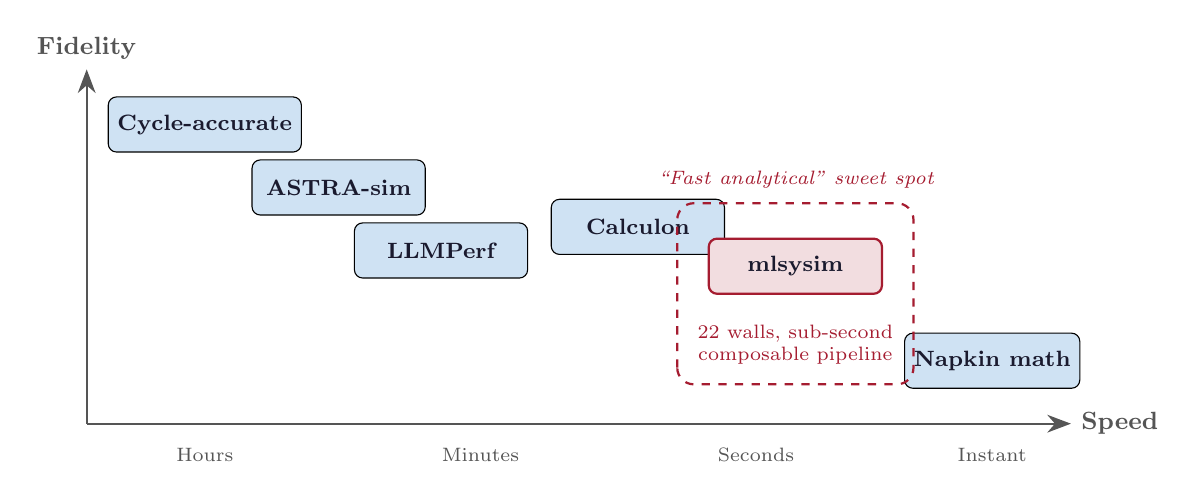
\begin{tikzpicture}[
  every node/.style={font=\small},
  arrow/.style={-{Stealth[length=3mm]}, thick, color=midgray},
  tool/.style={draw, rounded corners=3pt, fill=computeblue, text=darktext,
               minimum height=0.7cm, minimum width=2.2cm, font=\footnotesize\bfseries},
  highlight/.style={tool, fill=crimson!15, draw=crimson, thick},
]
  % Axis
  \draw[arrow] (0,0) -- (12.5,0) node[right] {\textbf{Speed}};
  \draw[arrow] (0,0) -- (0,4.5)  node[above] {\textbf{Fidelity}};

  % Labels on axis
  \node[font=\scriptsize, color=midgray] at (1.5,-0.4) {Hours};
  \node[font=\scriptsize, color=midgray] at (5.0,-0.4) {Minutes};
  \node[font=\scriptsize, color=midgray] at (8.5,-0.4) {Seconds};
  \node[font=\scriptsize, color=midgray] at (11.5,-0.4) {Instant};

  % Tools
  \node[tool] (cycle) at (1.5, 3.8) {Cycle-accurate};
  \node[tool] (astra) at (3.2, 3.0) {ASTRA-sim};
  \node[tool] (llmperf) at (4.5, 2.2) {LLMPerf};
  \node[tool] (calculon) at (7.0, 2.5) {Calculon};
  \node[highlight] (mlsysim) at (9.0, 2.0) {mlsysim};
  \node[tool] (napkin) at (11.5, 0.8) {Napkin math};

  % Annotation for mlsysim
  \node[font=\scriptsize, color=crimson, align=center] at (9.0, 1.0)
    {22 walls, sub-second\\composable pipeline};

  % Sweet-spot region
  \draw[dashed, crimson, thick, rounded corners=6pt]
    (7.5, 0.5) rectangle (10.5, 2.8);
  \node[font=\scriptsize\itshape, color=crimson] at (9.0, 3.1)
    {``Fast analytical'' sweet spot};
\end{tikzpicture}

\vspace{0.3em}
\small\itshape
mlsysim trades cycle-accuracy for speed and breadth.\\
The right tool depends on the question you are asking.
\end{frame}

% --- Slide R.4: What mlsysim Does NOT Do ---
\begin{frame}{What mlsysim Does NOT Do}
\begin{columns}[T]
\column{0.52\textwidth}
\textbf{\textcolor{crimson}{Not a replacement for:}}
\begin{itemize}
  \item \textbf{Benchmarking} --- real measurements on real hardware
  \item \textbf{Cycle-accurate simulation} --- microarchitectural detail
  \item \textbf{Production deployment} --- no orchestration, no serving
  \item \textbf{Framework profiling} --- no kernel-level tracing
\end{itemize}

\vspace{0.5em}
\textbf{Prediction accuracy:}\\
Within \alert{2--5$\times$} of measured performance.\\
Useful for \emph{ranking} and \emph{bounding},\\
not for exact latency guarantees.

\column{0.45\textwidth}
\textbf{\textcolor{datastroke}{What it IS:}}
\begin{itemize}
  \item A \textbf{reasoning framework}
  \item Answers ``which constraint binds?''
  \item Answers ``is this hardware sufficient?''
  \item Answers ``what should I try first?''
  \item Runs in $<$1\,ms per evaluation
  \item No GPU required
\end{itemize}

\vspace{0.5em}
\begin{center}
\small\itshape
``All models are wrong,\\
but some are useful.''\\
--- George Box
\end{center}
\end{columns}
\end{frame}

% --- Slide R.5: How to Think About Accuracy ---
\begin{frame}{How to Think About Accuracy: The CPI Analogy}
\begin{block}{Patterson's Insight (Computer Architecture)}
\small
Hennessy \& Patterson did not predict CPI from first principles.\\
They \textbf{measured} CPI empirically, then used it to \textbf{reason} about
architectural tradeoffs. The value was in the \textbf{framework}, not the exact number.
\end{block}

\vspace{0.5em}
\begin{block}{Our Approach (ML Systems)}
\small
We do not predict $\eta$ (efficiency) from first principles.\\
We \textbf{measure} $\eta$ empirically (MFU from published papers), then use it
to \textbf{reason} about system tradeoffs across 22 walls.
\end{block}

\vspace{0.8em}
\centering
\begin{tabular}{@{}lll@{}}
\toprule
& \textbf{Computer Architecture} & \textbf{ML Systems} \\
\midrule
Empirical constant & CPI & $\eta$ (MFU) \\
Framework & Iron Law of CPU Perf & Iron Law of ML Systems \\
Value & Reason about ISA tradeoffs & Reason about system walls \\
\bottomrule
\end{tabular}
\end{frame}

% --- Slide R.6: The Iron Law --- Our Contribution ---
\begin{frame}{The Iron Law: Every Wall Maps to a Term}
\begin{center}
\large
\[
T = \frac{\text{FLOPs}}{N \;\times\; \text{Peak} \;\times\; \text{MFU} \;\times\; \eta_{\text{scaling}} \;\times\; \text{Goodput}}
\]
\end{center}

\vspace{0.3em}
\small
\begin{columns}[T]
\column{0.48\textwidth}
\begin{tabular}{@{}ll@{}}
\toprule
\textbf{Term} & \textbf{Walls} \\
\midrule
FLOPs (numerator) & 11 Complexity \\
                   & 12 Reasoning \\
                   & 13 Fidelity \\
\midrule
$N$ (parallelism)  & 14 Communication \\
                   & 15 Fragility \\
                   & 16 Multi-tenant \\
\bottomrule
\end{tabular}

\column{0.48\textwidth}
\begin{tabular}{@{}ll@{}}
\toprule
\textbf{Term} & \textbf{Walls} \\
\midrule
Peak (hardware) & 1 Compute \\
                & 2 Memory \\
                & 6 Streaming \\
\midrule
MFU (efficiency) & 3 Software \\
                 & 4 Serving \\
                 & 5 Batching \\
\midrule
Goodput          & 8 Ingestion \\
                 & 9 Transformation \\
                 & 19 Checkpoint \\
\bottomrule
\end{tabular}
\end{columns}

\vspace{0.5em}
\centering
\footnotesize
Remaining walls: 7 Tail Latency, 10 Locality, 17 Capital, 18 Sustainability, 20 Safety, 21 Sensitivity, 22 Synthesis\\
These are \textbf{cross-cutting constraints} and \textbf{meta-analysis tools} that modulate the Iron Law terms.
\end{frame}

% --- Slide R.7: 22 Walls at a Glance ---
\begin{frame}{22 Walls at a Glance}
\centering
\scriptsize
\setlength{\tabcolsep}{3pt}
\begin{tabular}{@{}rllll@{}}
\toprule
\textbf{\#} & \textbf{Wall} & \textbf{Domain} & \textbf{Constraint} & \textbf{Key Equation} \\
\midrule
1  & Compute       & Node      & Peak FLOPS ceiling            & $T = \text{OPs} / (\text{Peak} \times \eta)$ \\
2  & Memory        & Node      & HBM capacity \& bandwidth     & $T = |W| / \text{BW}$ \\
3  & Software      & Node      & Peak vs achieved FLOPS        & $\eta_{\text{MFU}}$ \\
4  & Serving       & Node      & Prefill vs decode regimes     & TTFT, ITL \\
5  & Batching      & Node      & KV cache fragmentation        & PagedAttention \\
6  & Streaming     & Node      & Injection BW (wafer-scale)    & $T = |W| / \text{BW}_{\text{inj}}$ \\
7  & Tail Latency  & Node      & P99 grows near saturation     & Erlang-C \\
\midrule
8  & Ingestion     & Data      & Storage I/O supply rate       & $\rho = \text{BW}_d / \text{BW}_s$ \\
9  & Transform     & Data      & CPU preprocessing rate        & $T = BS / C$ \\
10 & Locality      & Data      & Bisection bandwidth limit     & $\text{BW}_{\text{eff}}$ \\
\midrule
11 & Complexity    & Algorithm & Chinchilla scaling laws       & $C = 6PD$ \\
12 & Reasoning     & Algorithm & Inference-time compute        & $T = K \times T_{\text{step}}$ \\
13 & Fidelity      & Algorithm & Compression--accuracy tradeoff & $r = 32/b$ \\
\midrule
14 & Communication & Fleet     & AllReduce synchronization     & Ring AllReduce \\
15 & Fragility     & Fleet     & Component failures at scale   & $\text{MTBF}/N$ \\
16 & Multi-tenant  & Fleet     & Queueing delays in shared clusters & $\rho / [2\mu(1{-}\rho)]$ \\
\midrule
17 & Capital       & Ops       & Total cost of ownership       & TCO = CapEx + OpEx \\
18 & Sustainability & Ops      & Carbon \& water footprint     & $\text{CO}_2 = E \times \text{PUE} \times \text{CI}$ \\
19 & Checkpoint    & Ops       & I/O burst penalty on MFU      & $T_w / T_i$ \\
20 & Safety        & Ops       & Privacy/fairness overhead     & DP-SGD $\sigma \propto 1/\varepsilon$ \\
\midrule
21 & Sensitivity   & Analysis  & Binding constraint ID         & $\partial T / \partial x_i$ \\
22 & Synthesis     & Analysis  & Inverse Roofline (HW from SLA) & $\text{BW} = |W| / T$ \\
\bottomrule
\end{tabular}
\end{frame}

% --- Slide R.8: Try It Now ---
\begin{frame}[fragile]{Try It Now}
\begin{center}
\Large\bfseries
One install. No GPU. Sub-second answers.
\end{center}

\vspace{1em}
\begin{lstlisting}[language=bash, backgroundcolor=\color{crimson!6}]
pip install mlsysim
\end{lstlisting}

\vspace{0.5em}
\begin{lstlisting}
import mlsysim

# Profile Llama-3 8B on H100 in one line
profile = mlsysim.Engine.solve(
    mlsysim.Models.Language.Llama3_8B,
    mlsysim.Hardware.H100,
    batch_size=1, seq_len=2048
)
print(profile.summary())
# => bottleneck, latency, throughput, MFU, feasibility
\end{lstlisting}

\vspace{0.5em}
\centering
\small
\begin{tabular}{@{}ll@{}}
GitHub:  & \texttt{github.com/harvard-edge/mlsysim} \\
Docs:    & \texttt{mlsysim.readthedocs.io} \\
Paper:   & \texttt{arxiv.org/abs/XXXX.XXXXX} \\
\end{tabular}
\end{frame}
 into tutorial_part1.tex
% or tutorial_part2.tex. It contains no preamble or document environment.
% =============================================================================

% =====================================================================
% RELATED WORK & POSITIONING
% =====================================================================
\section{Related Work}

% --- Slide R.1: The Landscape ---
\begin{frame}{The Landscape: Existing ML Performance Tools}
\centering
\scriptsize
\begin{tabular}{@{}llllll@{}}
\toprule
\textbf{Tool} & \textbf{Type} & \textbf{Speed} & \textbf{Scope} & \textbf{Access} \\
\midrule
ASTRA-sim        & Discrete-event   & Hours      & Network              & Open \\
Calculon         & Analytical       & Seconds    & Training             & Open \\
DeepSpeed Profiler & Runtime        & Real-time  & Single-node          & Requires GPU \\
LLMPerf / vLLM   & Empirical        & Minutes    & Serving              & Requires GPU \\
Roofline Toolkit  & Empirical        & Minutes    & Compute/memory       & Requires HW \\
Internal (Google, Meta) & Analytical & Seconds    & Full-stack           & Proprietary \\
\rowcolor{crimson!12}
\textbf{mlsysim} & \textbf{Analytical} & \textbf{Sub-second} & \textbf{22 walls} & \textbf{Open, no GPU} \\
\bottomrule
\end{tabular}

\vspace{0.8em}
\small
\textbf{Key observation:} Open tools cover 3--4 constraints each.\\
No existing open tool covers the full stack from compute to carbon.
\end{frame}

% --- Slide R.2: What Makes mlsysim Different? ---
\begin{frame}{What Makes mlsysim Different?}
\begin{columns}[T]
\column{0.55\textwidth}
\begin{enumerate}
  \item \textbf{Breadth: 22 walls in one pipeline}\\
    \small Others cover 3--4 constraints.\\
    mlsysim composes all 22 into a single\\
    \texttt{Pipeline.solve()} call.

  \vspace{0.6em}
  \item \textbf{Unit safety: Pint dimensional analysis}\\
    \small Every quantity carries its unit.\\
    \texttt{GB + TFLOPS} $\Rightarrow$ \textcolor{crimson}{DimensionalityError}.\\
    Catches errors spreadsheets never will.

  \vspace{0.6em}
  \item \textbf{Traceability: Every constant is cited}\\
    \small \texttt{TraceableConstant} records source,\\
    date, and DOI for every hardware spec.\\
    Audit any number back to its origin.
\end{enumerate}

\column{0.42\textwidth}
\centering
\begin{block}{The Trifecta}
\small
\begin{tabular}{@{}lc@{}}
Feature & Others \\
\midrule
22 walls     & 3--4 \\
Unit safety  & None \\
Traceability & Rare \\
\end{tabular}
\end{block}

\vspace{1em}
\begin{exampleblock}{One-Liner}
\footnotesize
\texttt{pip install mlsysim}\\[2pt]
No GPU. No cluster.\\
Just Python 3.10+.
\end{exampleblock}
\end{columns}
\end{frame}

% --- Slide R.3: The Fidelity-Speed Spectrum ---
\begin{frame}{The Fidelity--Speed Spectrum}
\centering
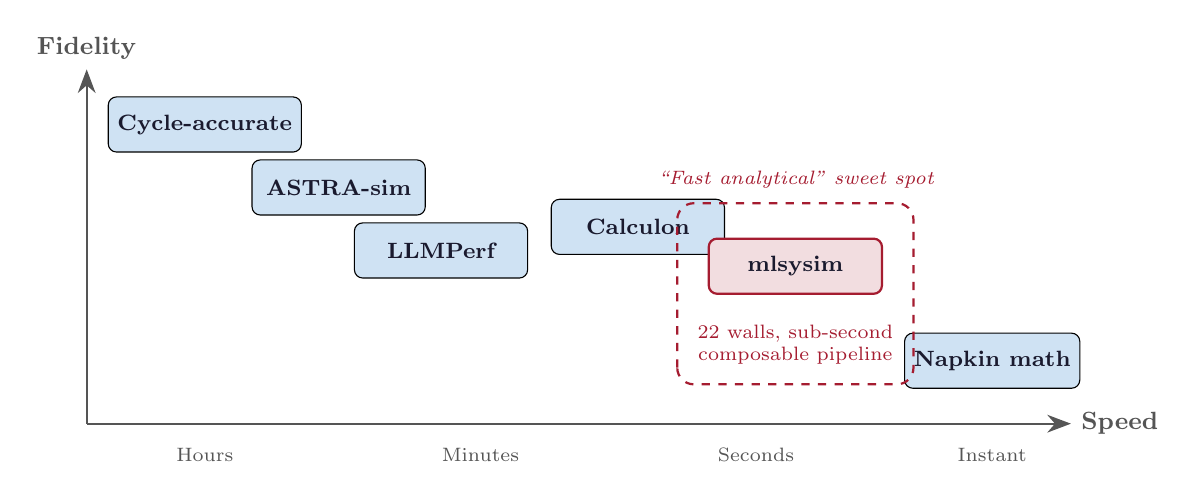
\begin{tikzpicture}[
  every node/.style={font=\small},
  arrow/.style={-{Stealth[length=3mm]}, thick, color=midgray},
  tool/.style={draw, rounded corners=3pt, fill=computeblue, text=darktext,
               minimum height=0.7cm, minimum width=2.2cm, font=\footnotesize\bfseries},
  highlight/.style={tool, fill=crimson!15, draw=crimson, thick},
]
  % Axis
  \draw[arrow] (0,0) -- (12.5,0) node[right] {\textbf{Speed}};
  \draw[arrow] (0,0) -- (0,4.5)  node[above] {\textbf{Fidelity}};

  % Labels on axis
  \node[font=\scriptsize, color=midgray] at (1.5,-0.4) {Hours};
  \node[font=\scriptsize, color=midgray] at (5.0,-0.4) {Minutes};
  \node[font=\scriptsize, color=midgray] at (8.5,-0.4) {Seconds};
  \node[font=\scriptsize, color=midgray] at (11.5,-0.4) {Instant};

  % Tools
  \node[tool] (cycle) at (1.5, 3.8) {Cycle-accurate};
  \node[tool] (astra) at (3.2, 3.0) {ASTRA-sim};
  \node[tool] (llmperf) at (4.5, 2.2) {LLMPerf};
  \node[tool] (calculon) at (7.0, 2.5) {Calculon};
  \node[highlight] (mlsysim) at (9.0, 2.0) {mlsysim};
  \node[tool] (napkin) at (11.5, 0.8) {Napkin math};

  % Annotation for mlsysim
  \node[font=\scriptsize, color=crimson, align=center] at (9.0, 1.0)
    {22 walls, sub-second\\composable pipeline};

  % Sweet-spot region
  \draw[dashed, crimson, thick, rounded corners=6pt]
    (7.5, 0.5) rectangle (10.5, 2.8);
  \node[font=\scriptsize\itshape, color=crimson] at (9.0, 3.1)
    {``Fast analytical'' sweet spot};
\end{tikzpicture}

\vspace{0.3em}
\small\itshape
mlsysim trades cycle-accuracy for speed and breadth.\\
The right tool depends on the question you are asking.
\end{frame}

% --- Slide R.4: What mlsysim Does NOT Do ---
\begin{frame}{What mlsysim Does NOT Do}
\begin{columns}[T]
\column{0.52\textwidth}
\textbf{\textcolor{crimson}{Not a replacement for:}}
\begin{itemize}
  \item \textbf{Benchmarking} --- real measurements on real hardware
  \item \textbf{Cycle-accurate simulation} --- microarchitectural detail
  \item \textbf{Production deployment} --- no orchestration, no serving
  \item \textbf{Framework profiling} --- no kernel-level tracing
\end{itemize}

\vspace{0.5em}
\textbf{Prediction accuracy:}\\
Within \alert{2--5$\times$} of measured performance.\\
Useful for \emph{ranking} and \emph{bounding},\\
not for exact latency guarantees.

\column{0.45\textwidth}
\textbf{\textcolor{datastroke}{What it IS:}}
\begin{itemize}
  \item A \textbf{reasoning framework}
  \item Answers ``which constraint binds?''
  \item Answers ``is this hardware sufficient?''
  \item Answers ``what should I try first?''
  \item Runs in $<$1\,ms per evaluation
  \item No GPU required
\end{itemize}

\vspace{0.5em}
\begin{center}
\small\itshape
``All models are wrong,\\
but some are useful.''\\
--- George Box
\end{center}
\end{columns}
\end{frame}

% --- Slide R.5: How to Think About Accuracy ---
\begin{frame}{How to Think About Accuracy: The CPI Analogy}
\begin{block}{Patterson's Insight (Computer Architecture)}
\small
Hennessy \& Patterson did not predict CPI from first principles.\\
They \textbf{measured} CPI empirically, then used it to \textbf{reason} about
architectural tradeoffs. The value was in the \textbf{framework}, not the exact number.
\end{block}

\vspace{0.5em}
\begin{block}{Our Approach (ML Systems)}
\small
We do not predict $\eta$ (efficiency) from first principles.\\
We \textbf{measure} $\eta$ empirically (MFU from published papers), then use it
to \textbf{reason} about system tradeoffs across 22 walls.
\end{block}

\vspace{0.8em}
\centering
\begin{tabular}{@{}lll@{}}
\toprule
& \textbf{Computer Architecture} & \textbf{ML Systems} \\
\midrule
Empirical constant & CPI & $\eta$ (MFU) \\
Framework & Iron Law of CPU Perf & Iron Law of ML Systems \\
Value & Reason about ISA tradeoffs & Reason about system walls \\
\bottomrule
\end{tabular}
\end{frame}

% --- Slide R.6: The Iron Law --- Our Contribution ---
\begin{frame}{The Iron Law: Every Wall Maps to a Term}
\begin{center}
\large
\[
T = \frac{\text{FLOPs}}{N \;\times\; \text{Peak} \;\times\; \text{MFU} \;\times\; \eta_{\text{scaling}} \;\times\; \text{Goodput}}
\]
\end{center}

\vspace{0.3em}
\small
\begin{columns}[T]
\column{0.48\textwidth}
\begin{tabular}{@{}ll@{}}
\toprule
\textbf{Term} & \textbf{Walls} \\
\midrule
FLOPs (numerator) & 11 Complexity \\
                   & 12 Reasoning \\
                   & 13 Fidelity \\
\midrule
$N$ (parallelism)  & 14 Communication \\
                   & 15 Fragility \\
                   & 16 Multi-tenant \\
\bottomrule
\end{tabular}

\column{0.48\textwidth}
\begin{tabular}{@{}ll@{}}
\toprule
\textbf{Term} & \textbf{Walls} \\
\midrule
Peak (hardware) & 1 Compute \\
                & 2 Memory \\
                & 6 Streaming \\
\midrule
MFU (efficiency) & 3 Software \\
                 & 4 Serving \\
                 & 5 Batching \\
\midrule
Goodput          & 8 Ingestion \\
                 & 9 Transformation \\
                 & 19 Checkpoint \\
\bottomrule
\end{tabular}
\end{columns}

\vspace{0.5em}
\centering
\footnotesize
Remaining walls: 7 Tail Latency, 10 Locality, 17 Capital, 18 Sustainability, 20 Safety, 21 Sensitivity, 22 Synthesis\\
These are \textbf{cross-cutting constraints} and \textbf{meta-analysis tools} that modulate the Iron Law terms.
\end{frame}

% --- Slide R.7: 22 Walls at a Glance ---
\begin{frame}{22 Walls at a Glance}
\centering
\scriptsize
\setlength{\tabcolsep}{3pt}
\begin{tabular}{@{}rllll@{}}
\toprule
\textbf{\#} & \textbf{Wall} & \textbf{Domain} & \textbf{Constraint} & \textbf{Key Equation} \\
\midrule
1  & Compute       & Node      & Peak FLOPS ceiling            & $T = \text{OPs} / (\text{Peak} \times \eta)$ \\
2  & Memory        & Node      & HBM capacity \& bandwidth     & $T = |W| / \text{BW}$ \\
3  & Software      & Node      & Peak vs achieved FLOPS        & $\eta_{\text{MFU}}$ \\
4  & Serving       & Node      & Prefill vs decode regimes     & TTFT, ITL \\
5  & Batching      & Node      & KV cache fragmentation        & PagedAttention \\
6  & Streaming     & Node      & Injection BW (wafer-scale)    & $T = |W| / \text{BW}_{\text{inj}}$ \\
7  & Tail Latency  & Node      & P99 grows near saturation     & Erlang-C \\
\midrule
8  & Ingestion     & Data      & Storage I/O supply rate       & $\rho = \text{BW}_d / \text{BW}_s$ \\
9  & Transform     & Data      & CPU preprocessing rate        & $T = BS / C$ \\
10 & Locality      & Data      & Bisection bandwidth limit     & $\text{BW}_{\text{eff}}$ \\
\midrule
11 & Complexity    & Algorithm & Chinchilla scaling laws       & $C = 6PD$ \\
12 & Reasoning     & Algorithm & Inference-time compute        & $T = K \times T_{\text{step}}$ \\
13 & Fidelity      & Algorithm & Compression--accuracy tradeoff & $r = 32/b$ \\
\midrule
14 & Communication & Fleet     & AllReduce synchronization     & Ring AllReduce \\
15 & Fragility     & Fleet     & Component failures at scale   & $\text{MTBF}/N$ \\
16 & Multi-tenant  & Fleet     & Queueing delays in shared clusters & $\rho / [2\mu(1{-}\rho)]$ \\
\midrule
17 & Capital       & Ops       & Total cost of ownership       & TCO = CapEx + OpEx \\
18 & Sustainability & Ops      & Carbon \& water footprint     & $\text{CO}_2 = E \times \text{PUE} \times \text{CI}$ \\
19 & Checkpoint    & Ops       & I/O burst penalty on MFU      & $T_w / T_i$ \\
20 & Safety        & Ops       & Privacy/fairness overhead     & DP-SGD $\sigma \propto 1/\varepsilon$ \\
\midrule
21 & Sensitivity   & Analysis  & Binding constraint ID         & $\partial T / \partial x_i$ \\
22 & Synthesis     & Analysis  & Inverse Roofline (HW from SLA) & $\text{BW} = |W| / T$ \\
\bottomrule
\end{tabular}
\end{frame}

% --- Slide R.8: Try It Now ---
\begin{frame}[fragile]{Try It Now}
\begin{center}
\Large\bfseries
One install. No GPU. Sub-second answers.
\end{center}

\vspace{1em}
\begin{lstlisting}[language=bash, backgroundcolor=\color{crimson!6}]
pip install mlsysim
\end{lstlisting}

\vspace{0.5em}
\begin{lstlisting}
import mlsysim

# Profile Llama-3 8B on H100 in one line
profile = mlsysim.Engine.solve(
    mlsysim.Models.Language.Llama3_8B,
    mlsysim.Hardware.H100,
    batch_size=1, seq_len=2048
)
print(profile.summary())
# => bottleneck, latency, throughput, MFU, feasibility
\end{lstlisting}

\vspace{0.5em}
\centering
\small
\begin{tabular}{@{}ll@{}}
GitHub:  & \texttt{github.com/harvard-edge/mlsysim} \\
Docs:    & \texttt{mlsysim.readthedocs.io} \\
Paper:   & \texttt{arxiv.org/abs/XXXX.XXXXX} \\
\end{tabular}
\end{frame}
 into tutorial_part1.tex
% or tutorial_part2.tex. It contains no preamble or document environment.
% =============================================================================

% =====================================================================
% RELATED WORK & POSITIONING
% =====================================================================
\section{Related Work}

% --- Slide R.1: The Landscape ---
\begin{frame}{The Landscape: Existing ML Performance Tools}
\centering
\scriptsize
\begin{tabular}{@{}llllll@{}}
\toprule
\textbf{Tool} & \textbf{Type} & \textbf{Speed} & \textbf{Scope} & \textbf{Access} \\
\midrule
ASTRA-sim        & Discrete-event   & Hours      & Network              & Open \\
Calculon         & Analytical       & Seconds    & Training             & Open \\
DeepSpeed Profiler & Runtime        & Real-time  & Single-node          & Requires GPU \\
LLMPerf / vLLM   & Empirical        & Minutes    & Serving              & Requires GPU \\
Roofline Toolkit  & Empirical        & Minutes    & Compute/memory       & Requires HW \\
Internal (Google, Meta) & Analytical & Seconds    & Full-stack           & Proprietary \\
\rowcolor{crimson!12}
\textbf{mlsysim} & \textbf{Analytical} & \textbf{Sub-second} & \textbf{22 walls} & \textbf{Open, no GPU} \\
\bottomrule
\end{tabular}

\vspace{0.8em}
\small
\textbf{Key observation:} Open tools cover 3--4 constraints each.\\
No existing open tool covers the full stack from compute to carbon.
\end{frame}

% --- Slide R.2: What Makes mlsysim Different? ---
\begin{frame}{What Makes mlsysim Different?}
\begin{columns}[T]
\column{0.55\textwidth}
\begin{enumerate}
  \item \textbf{Breadth: 22 walls in one pipeline}\\
    \small Others cover 3--4 constraints.\\
    mlsysim composes all 22 into a single\\
    \texttt{Pipeline.solve()} call.

  \vspace{0.6em}
  \item \textbf{Unit safety: Pint dimensional analysis}\\
    \small Every quantity carries its unit.\\
    \texttt{GB + TFLOPS} $\Rightarrow$ \textcolor{crimson}{DimensionalityError}.\\
    Catches errors spreadsheets never will.

  \vspace{0.6em}
  \item \textbf{Traceability: Every constant is cited}\\
    \small \texttt{TraceableConstant} records source,\\
    date, and DOI for every hardware spec.\\
    Audit any number back to its origin.
\end{enumerate}

\column{0.42\textwidth}
\centering
\begin{block}{The Trifecta}
\small
\begin{tabular}{@{}lc@{}}
Feature & Others \\
\midrule
22 walls     & 3--4 \\
Unit safety  & None \\
Traceability & Rare \\
\end{tabular}
\end{block}

\vspace{1em}
\begin{exampleblock}{One-Liner}
\footnotesize
\texttt{pip install mlsysim}\\[2pt]
No GPU. No cluster.\\
Just Python 3.10+.
\end{exampleblock}
\end{columns}
\end{frame}

% --- Slide R.3: The Fidelity-Speed Spectrum ---
\begin{frame}{The Fidelity--Speed Spectrum}
\centering
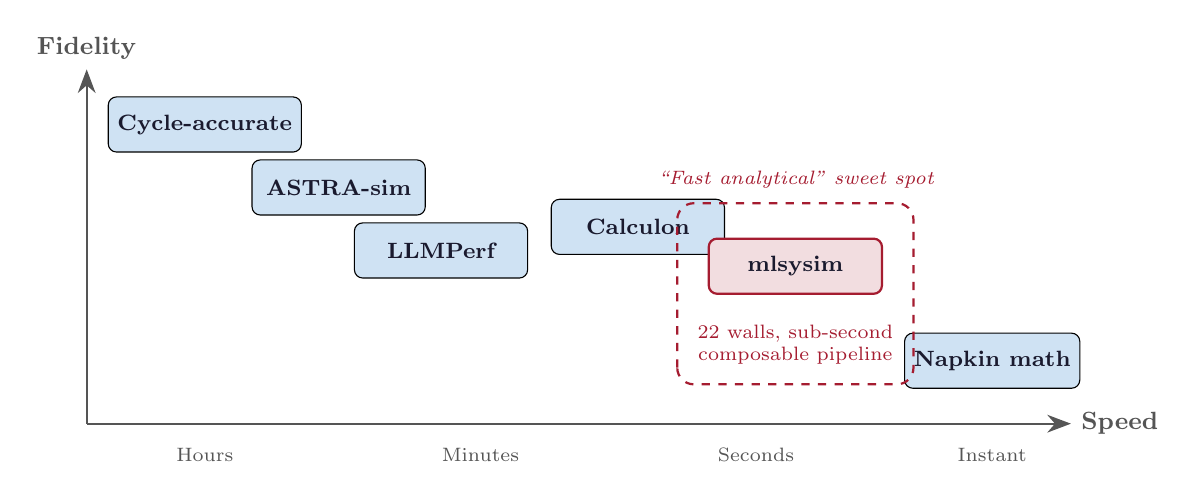
\begin{tikzpicture}[
  every node/.style={font=\small},
  arrow/.style={-{Stealth[length=3mm]}, thick, color=midgray},
  tool/.style={draw, rounded corners=3pt, fill=computeblue, text=darktext,
               minimum height=0.7cm, minimum width=2.2cm, font=\footnotesize\bfseries},
  highlight/.style={tool, fill=crimson!15, draw=crimson, thick},
]
  % Axis
  \draw[arrow] (0,0) -- (12.5,0) node[right] {\textbf{Speed}};
  \draw[arrow] (0,0) -- (0,4.5)  node[above] {\textbf{Fidelity}};

  % Labels on axis
  \node[font=\scriptsize, color=midgray] at (1.5,-0.4) {Hours};
  \node[font=\scriptsize, color=midgray] at (5.0,-0.4) {Minutes};
  \node[font=\scriptsize, color=midgray] at (8.5,-0.4) {Seconds};
  \node[font=\scriptsize, color=midgray] at (11.5,-0.4) {Instant};

  % Tools
  \node[tool] (cycle) at (1.5, 3.8) {Cycle-accurate};
  \node[tool] (astra) at (3.2, 3.0) {ASTRA-sim};
  \node[tool] (llmperf) at (4.5, 2.2) {LLMPerf};
  \node[tool] (calculon) at (7.0, 2.5) {Calculon};
  \node[highlight] (mlsysim) at (9.0, 2.0) {mlsysim};
  \node[tool] (napkin) at (11.5, 0.8) {Napkin math};

  % Annotation for mlsysim
  \node[font=\scriptsize, color=crimson, align=center] at (9.0, 1.0)
    {22 walls, sub-second\\composable pipeline};

  % Sweet-spot region
  \draw[dashed, crimson, thick, rounded corners=6pt]
    (7.5, 0.5) rectangle (10.5, 2.8);
  \node[font=\scriptsize\itshape, color=crimson] at (9.0, 3.1)
    {``Fast analytical'' sweet spot};
\end{tikzpicture}

\vspace{0.3em}
\small\itshape
mlsysim trades cycle-accuracy for speed and breadth.\\
The right tool depends on the question you are asking.
\end{frame}

% --- Slide R.4: What mlsysim Does NOT Do ---
\begin{frame}{What mlsysim Does NOT Do}
\begin{columns}[T]
\column{0.52\textwidth}
\textbf{\textcolor{crimson}{Not a replacement for:}}
\begin{itemize}
  \item \textbf{Benchmarking} --- real measurements on real hardware
  \item \textbf{Cycle-accurate simulation} --- microarchitectural detail
  \item \textbf{Production deployment} --- no orchestration, no serving
  \item \textbf{Framework profiling} --- no kernel-level tracing
\end{itemize}

\vspace{0.5em}
\textbf{Prediction accuracy:}\\
Within \alert{2--5$\times$} of measured performance.\\
Useful for \emph{ranking} and \emph{bounding},\\
not for exact latency guarantees.

\column{0.45\textwidth}
\textbf{\textcolor{datastroke}{What it IS:}}
\begin{itemize}
  \item A \textbf{reasoning framework}
  \item Answers ``which constraint binds?''
  \item Answers ``is this hardware sufficient?''
  \item Answers ``what should I try first?''
  \item Runs in $<$1\,ms per evaluation
  \item No GPU required
\end{itemize}

\vspace{0.5em}
\begin{center}
\small\itshape
``All models are wrong,\\
but some are useful.''\\
--- George Box
\end{center}
\end{columns}
\end{frame}

% --- Slide R.5: How to Think About Accuracy ---
\begin{frame}{How to Think About Accuracy: The CPI Analogy}
\begin{block}{Patterson's Insight (Computer Architecture)}
\small
Hennessy \& Patterson did not predict CPI from first principles.\\
They \textbf{measured} CPI empirically, then used it to \textbf{reason} about
architectural tradeoffs. The value was in the \textbf{framework}, not the exact number.
\end{block}

\vspace{0.5em}
\begin{block}{Our Approach (ML Systems)}
\small
We do not predict $\eta$ (efficiency) from first principles.\\
We \textbf{measure} $\eta$ empirically (MFU from published papers), then use it
to \textbf{reason} about system tradeoffs across 22 walls.
\end{block}

\vspace{0.8em}
\centering
\begin{tabular}{@{}lll@{}}
\toprule
& \textbf{Computer Architecture} & \textbf{ML Systems} \\
\midrule
Empirical constant & CPI & $\eta$ (MFU) \\
Framework & Iron Law of CPU Perf & Iron Law of ML Systems \\
Value & Reason about ISA tradeoffs & Reason about system walls \\
\bottomrule
\end{tabular}
\end{frame}

% --- Slide R.6: The Iron Law --- Our Contribution ---
\begin{frame}{The Iron Law: Every Wall Maps to a Term}
\begin{center}
\large
\[
T = \frac{\text{FLOPs}}{N \;\times\; \text{Peak} \;\times\; \text{MFU} \;\times\; \eta_{\text{scaling}} \;\times\; \text{Goodput}}
\]
\end{center}

\vspace{0.3em}
\small
\begin{columns}[T]
\column{0.48\textwidth}
\begin{tabular}{@{}ll@{}}
\toprule
\textbf{Term} & \textbf{Walls} \\
\midrule
FLOPs (numerator) & 11 Complexity \\
                   & 12 Reasoning \\
                   & 13 Fidelity \\
\midrule
$N$ (parallelism)  & 14 Communication \\
                   & 15 Fragility \\
                   & 16 Multi-tenant \\
\bottomrule
\end{tabular}

\column{0.48\textwidth}
\begin{tabular}{@{}ll@{}}
\toprule
\textbf{Term} & \textbf{Walls} \\
\midrule
Peak (hardware) & 1 Compute \\
                & 2 Memory \\
                & 6 Streaming \\
\midrule
MFU (efficiency) & 3 Software \\
                 & 4 Serving \\
                 & 5 Batching \\
\midrule
Goodput          & 8 Ingestion \\
                 & 9 Transformation \\
                 & 19 Checkpoint \\
\bottomrule
\end{tabular}
\end{columns}

\vspace{0.5em}
\centering
\footnotesize
Remaining walls: 7 Tail Latency, 10 Locality, 17 Capital, 18 Sustainability, 20 Safety, 21 Sensitivity, 22 Synthesis\\
These are \textbf{cross-cutting constraints} and \textbf{meta-analysis tools} that modulate the Iron Law terms.
\end{frame}

% --- Slide R.7: 22 Walls at a Glance ---
\begin{frame}{22 Walls at a Glance}
\centering
\scriptsize
\setlength{\tabcolsep}{3pt}
\begin{tabular}{@{}rllll@{}}
\toprule
\textbf{\#} & \textbf{Wall} & \textbf{Domain} & \textbf{Constraint} & \textbf{Key Equation} \\
\midrule
1  & Compute       & Node      & Peak FLOPS ceiling            & $T = \text{OPs} / (\text{Peak} \times \eta)$ \\
2  & Memory        & Node      & HBM capacity \& bandwidth     & $T = |W| / \text{BW}$ \\
3  & Software      & Node      & Peak vs achieved FLOPS        & $\eta_{\text{MFU}}$ \\
4  & Serving       & Node      & Prefill vs decode regimes     & TTFT, ITL \\
5  & Batching      & Node      & KV cache fragmentation        & PagedAttention \\
6  & Streaming     & Node      & Injection BW (wafer-scale)    & $T = |W| / \text{BW}_{\text{inj}}$ \\
7  & Tail Latency  & Node      & P99 grows near saturation     & Erlang-C \\
\midrule
8  & Ingestion     & Data      & Storage I/O supply rate       & $\rho = \text{BW}_d / \text{BW}_s$ \\
9  & Transform     & Data      & CPU preprocessing rate        & $T = BS / C$ \\
10 & Locality      & Data      & Bisection bandwidth limit     & $\text{BW}_{\text{eff}}$ \\
\midrule
11 & Complexity    & Algorithm & Chinchilla scaling laws       & $C = 6PD$ \\
12 & Reasoning     & Algorithm & Inference-time compute        & $T = K \times T_{\text{step}}$ \\
13 & Fidelity      & Algorithm & Compression--accuracy tradeoff & $r = 32/b$ \\
\midrule
14 & Communication & Fleet     & AllReduce synchronization     & Ring AllReduce \\
15 & Fragility     & Fleet     & Component failures at scale   & $\text{MTBF}/N$ \\
16 & Multi-tenant  & Fleet     & Queueing delays in shared clusters & $\rho / [2\mu(1{-}\rho)]$ \\
\midrule
17 & Capital       & Ops       & Total cost of ownership       & TCO = CapEx + OpEx \\
18 & Sustainability & Ops      & Carbon \& water footprint     & $\text{CO}_2 = E \times \text{PUE} \times \text{CI}$ \\
19 & Checkpoint    & Ops       & I/O burst penalty on MFU      & $T_w / T_i$ \\
20 & Safety        & Ops       & Privacy/fairness overhead     & DP-SGD $\sigma \propto 1/\varepsilon$ \\
\midrule
21 & Sensitivity   & Analysis  & Binding constraint ID         & $\partial T / \partial x_i$ \\
22 & Synthesis     & Analysis  & Inverse Roofline (HW from SLA) & $\text{BW} = |W| / T$ \\
\bottomrule
\end{tabular}
\end{frame}

% --- Slide R.8: Try It Now ---
\begin{frame}[fragile]{Try It Now}
\begin{center}
\Large\bfseries
One install. No GPU. Sub-second answers.
\end{center}

\vspace{1em}
\begin{lstlisting}[language=bash, backgroundcolor=\color{crimson!6}]
pip install mlsysim
\end{lstlisting}

\vspace{0.5em}
\begin{lstlisting}
import mlsysim

# Profile Llama-3 8B on H100 in one line
profile = mlsysim.Engine.solve(
    mlsysim.Models.Language.Llama3_8B,
    mlsysim.Hardware.H100,
    batch_size=1, seq_len=2048
)
print(profile.summary())
# => bottleneck, latency, throughput, MFU, feasibility
\end{lstlisting}

\vspace{0.5em}
\centering
\small
\begin{tabular}{@{}ll@{}}
GitHub:  & \texttt{github.com/harvard-edge/mlsysim} \\
Docs:    & \texttt{mlsysim.readthedocs.io} \\
Paper:   & \texttt{arxiv.org/abs/XXXX.XXXXX} \\
\end{tabular}
\end{frame}


% --- Roadmap: You Are Here (Morning) ---
\begin{frame}{Roadmap: You Are Here}
\note{[1 min] Quick orientation. We just finished the setup. Now the real work begins.}

\centering\small
\begin{tabular}{rll}
\toprule
\textbf{Time} & \textbf{Part} & \textbf{Status} \\
\midrule
9:00--9:30   & Part 0: Welcome \& Setup     & \checkmark Done \\
\rowcolor{crimson!12}
9:30--10:30  & \textbf{Part 1: Iron Law \& Roofline} & \textbf{$\leftarrow$ You are here} \\
10:45--11:45 & Part 2: Memory Walls \& Serving & \\
11:45--12:00 & Part 3: Compression & \\
\midrule
\textit{12:00--1:00} & \textit{Lunch} & \\
\midrule
1:00--2:15   & Part 4: Going Distributed & \\
2:30--3:15   & Part 5: Economics \& Sustainability & \\
3:15--3:45   & Part 6: Design Space Exploration & \\
3:45--4:15   & Part 7: TinyML to Frontier & \\
4:15--4:45   & Part 8: Advanced Topics & \\
4:45--5:00   & Part 9: Wrap-Up \& Capstone & \\
\bottomrule
\end{tabular}
\end{frame}

% =============================================================================
% PART 1: THE IRON LAW & ROOFLINE (15 slides)
% =============================================================================
\section{Iron Law \& Roofline}

% --- Slide 1.1: Key Question ---
\begin{frame}{Key Question}
\note{[1 min] Pose the question dramatically. Pause for 5 seconds.
``This is the most important question in ML systems engineering.
By the end of this section you will answer it in 3 lines of Python.''
% -- FLEX: [CORE]
}

\centering
\Large\bfseries
Why doesn't doubling FLOPS\\[0.3cm]
double your throughput?
\end{frame}

% --- Slide 1.2: Constraints Drive Architecture ---
\begin{frame}{Constraints Drive Architecture}
\note{[2 min] ``You don't choose a Transformer because it's trendy;
you choose it because of how it parallelizes on real silicon.
AI is not magic --- it is infrastructure, and infrastructure has laws.''
% -- FLEX: [CORE]
}

\small
\begin{itemize}
  \item Hardware has \textbf{finite compute} (FLOPS), \textbf{finite bandwidth}
        (GB/s), and \textbf{finite memory} (GB).
  \item Every workload demands some amount of each.
  \item The \textbf{binding constraint} is the one that takes the longest.
  \item \alert{You optimize the bottleneck, not the fast part.}
\end{itemize}

\vspace{0.5cm}
\centering
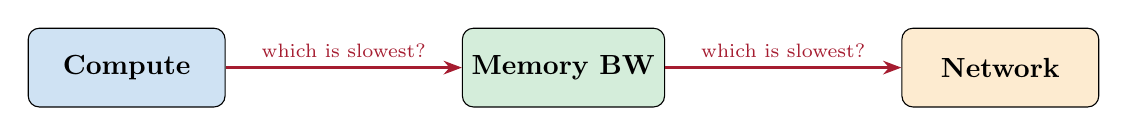
\begin{tikzpicture}[>=Stealth, node distance=3cm]
  \node[draw, fill=computeblue, rounded corners, minimum width=2.5cm, minimum height=1cm]
    (compute) {\textbf{Compute}};
  \node[draw, fill=datagreen, rounded corners, minimum width=2.5cm, minimum height=1cm,
    right=of compute] (memory) {\textbf{Memory BW}};
  \node[draw, fill=routingorange, rounded corners, minimum width=2.5cm, minimum height=1cm,
    right=of memory] (network) {\textbf{Network}};
  \draw[->, thick, crimson] (compute) -- node[above, font=\scriptsize] {which is slowest?} (memory);
  \draw[->, thick, crimson] (memory) -- node[above, font=\scriptsize] {which is slowest?} (network);
\end{tikzpicture}
\end{frame}

% --- Slide 1.3: The Roofline Model ---
\begin{frame}{The Roofline Model (Williams et al., 2009)}
\note{[3 min] Draw the two regimes on the board. Left = memory-bound,
right = compute-bound. The ridge point is where they cross.
``Before I show numbers: if a model does 16B FLOPs and
loads 16 GB of weights, what is its arithmetic intensity?''
Expected: 1 FLOP/byte. That is far left on the Roofline.
WARN: Students conflate FLOPS with throughput.
% -- FLEX: [CORE]
}

\small
\[
\text{Attainable FLOPS} = \min\!\bigl(\text{Peak FLOPS},\;\;
\text{BW} \times \text{Arithmetic Intensity}\bigr)
\]

\vspace{0.2cm}
\begin{columns}[T]
\begin{column}{0.55\textwidth}
\textbf{Arithmetic Intensity} (AI):
\[
  \text{AI} = \frac{\text{FLOPs}}{\text{Bytes moved}}
  \;\;\bigl[\text{FLOP/byte}\bigr]
\]

\vspace{0.2cm}
\begin{itemize}\setlength\itemsep{2pt}
  \item \textbf{AI $<$ Ridge Point} $\Rightarrow$ \colorbox{datagreen}{Memory-bound}
  \item \textbf{AI $>$ Ridge Point} $\Rightarrow$ \colorbox{computeblue}{Compute-bound}
\end{itemize}

\vspace{0.2cm}
Ridge Point $=$ Peak FLOPS $/$ Peak BW
\end{column}

\begin{column}{0.42\textwidth}
\centering
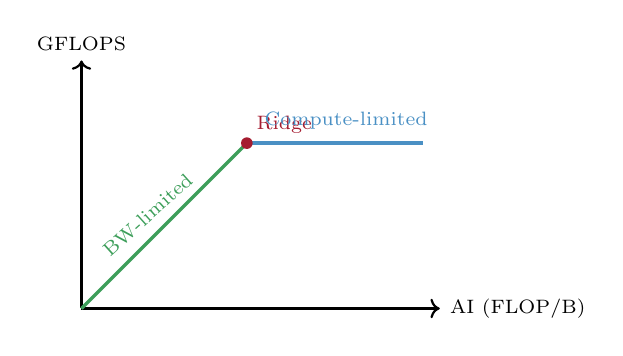
\begin{tikzpicture}[scale=0.7]
  % axes
  \draw[->, thick] (0,0) -- (6.5,0) node[right, font=\scriptsize] {AI (FLOP/B)};
  \draw[->, thick] (0,0) -- (0,4.5) node[above, font=\scriptsize] {GFLOPS};
  % memory roof
  \draw[very thick, datastroke] (0,0) -- (3,3);
  % compute roof
  \draw[very thick, computestroke] (3,3) -- (6.2,3);
  % ridge point
  \fill[crimson] (3,3) circle (3pt);
  \node[above right, font=\scriptsize, crimson] at (3,3) {Ridge};
  % labels
  \node[font=\scriptsize, datastroke, rotate=42] at (1.2,1.7) {BW-limited};
  \node[font=\scriptsize, computestroke] at (4.8,3.4) {Compute-limited};
\end{tikzpicture}
\end{column}
\end{columns}
\end{frame}

% --- Slide 1.4: The Compute Wall ---
\begin{frame}{Wall 1: The Compute Wall}
\note{[2 min] ``This is the speed limit. No software trick can make
your model run faster than the chip can crunch numbers.''
% -- FLEX: [CORE]
}

\small
\wallbox{The Compute Wall}{
\[
  T_{\text{compute}} = \frac{\text{Operations}}{\text{Peak FLOPS} \times \text{Efficiency}}
\]
}

\vspace{0.2cm}
\textbf{Example:} ResNet-50 inference at batch 256 on H100

\begin{itemize}
  \item FLOPs = $8.0 \times 10^{9} \times 256 = 2.05 \times 10^{12}$
  \item H100 FP16 Peak = 989 TFLOPS
  \item At 50\% MFU: $T = \frac{2.05 \times 10^{12}}{989 \times 10^{12} \times 0.5} \approx 4.1\;\text{ms}$
\end{itemize}

\vspace{0.2cm}
\alert{The chip is the ceiling. MFU is how close you get to it.}
\end{frame}

% --- Slide 1.5: The Memory Wall ---
\begin{frame}{Wall 2: The Memory Wall}
\note{[2 min] ``Quick mental math: 16 GB model, 3.35 TB/s bandwidth.
How long to load?'' Give 10 seconds. Expected: 16/3350 = 4.8 ms.
WARN: Students assume compute is always the bottleneck because
GPUs are marketed on TFLOPS.
% -- FLEX: [CORE]
}

\small
\wallbox{The Memory Wall}{
\[
  T_{\text{memory}} = \frac{\text{Weight Bytes}}{\text{Memory Bandwidth}}
\]
}

\vspace{0.2cm}
\textbf{Example:} Llama-3 8B at batch size 1 on H100

\begin{itemize}
  \item Weight size (FP16) = $8\text{B} \times 2\;\text{bytes} = 16\;\text{GB}$
  \item H100 HBM3 BW = 3.35 TB/s
  \item $T = \frac{16}{3350} \approx 4.8\;\text{ms}$ just to load weights
  \item Meanwhile, compute finishes in $\sim$0.03 ms
\end{itemize}

\vspace{0.2cm}
\alert{At batch size 1, LLM inference is $\sim$\,160$\times$ memory-bound.}
\end{frame}

% --- Slide 1.6: Predict Before You Peek #1 ---
\begin{frame}{Predict: H100 vs MI300X vs Gaudi\,3}
\note{[3 min] PREDICTION. Give the audience 60 seconds to think.
Expected answer: all memory-bound. BW ratios determine speedup, not FLOPS.
After the reveal, hammer home: ``The bottleneck determines the speedup.''
Turn to your neighbor: did you get the same answer? Why or why not? 60 seconds.
% -- FLEX: [CORE]
}

\centering
\Large\bfseries
Three flagship accelerators. Same workload.\\[0.3cm]
\normalsize
Llama-3 8B, batch size 1, FP16 inference.\\
Which is fastest---and by how much?\\[0.3cm]

\pause

\scriptsize
\begin{tabular}{lccc}
\toprule
              & \textbf{H100 (NVIDIA)} & \textbf{MI300X (AMD)} & \textbf{Gaudi\,3 (Intel)} \\
\midrule
Peak FP16     & 989 TFLOPS    & 1,307 TFLOPS  & 1,835 TFLOPS \\
HBM BW        & 3.35 TB/s     & 5.3 TB/s      & 3.7 TB/s \\
HBM Capacity  & 80 GB         & 192 GB        & 128 GB \\
\midrule
Bottleneck    & Memory        & Memory        & Memory \\
Weight-load time & 4.8 ms     & 3.0 ms        & 4.3 ms \\
\textbf{Speedup vs H100} & ---  & \textbf{1.6$\times$} & \textbf{1.1$\times$} \\
\bottomrule
\end{tabular}

\vspace{0.3cm}
\pause
\small
\alert{MI300X has fewer FLOPS than Gaudi\,3 but wins on bandwidth.\\
FLOPS don't determine speed when memory-bound.}
\end{frame}

% --- Slide 1.7: Live Demo --- Engine.solve (multi-vendor) ---
\begin{frame}[fragile]{Live Demo: Three Vendors, One API}
\note{[3 min] Run this live. The key moment: all three are memory-bound.
The ranking follows bandwidth, not FLOPS. This is ISCA---show that
mlsysim is not an NVIDIA-only tool.
% -- FLEX: [CORE]
}

\small
Run this in your Python session:

\begin{lstlisting}
import mlsysim

model = mlsysim.Models.Language.Llama3_8B
for hw_name in ["H100", "MI300X", "Gaudi3"]:
    hw = getattr(mlsysim.Hardware.Cloud, hw_name)
    p = mlsysim.Engine.solve(model, hw, batch_size=1)
    print(f"{hw.name}: {p.bottleneck}, "
          f"{p.latency:.2f}")
\end{lstlisting}

\vspace{0.2cm}
\begin{exampleblock}{What to look for}
  \begin{itemize}
    \item \texttt{bottleneck}: Memory for \textbf{all three}
    \item Ranking follows BW (MI300X $>$ Gaudi\,3 $>$ H100), not FLOPS
    \item Same API, same physics, different silicon
  \end{itemize}
\end{exampleblock}
\end{frame}

% --- Slide 1.8: MFU --- The Software Wall ---
\begin{frame}{Wall 3: MFU --- The Software Wall}
\note{[2 min] ``MFU measures the gap between what the hardware could do
and what your software actually achieves. A 50\% MFU means you are
paying for twice the hardware you are using.''
% -- FLEX: [CORE]
}

\small
\wallbox{Model FLOPs Utilization}{
\[
  \text{MFU} = \frac{\text{Achieved FLOPS}}{\text{Peak FLOPS}}
\]
}

\vspace{0.2cm}
\begin{columns}[T]
\begin{column}{0.55\textwidth}
\textbf{What eats MFU?}
\begin{itemize}\setlength\itemsep{2pt}
  \item Kernel launch overhead
  \item Memory stalls (cache misses)
  \item Framework overhead (Python $\to$ CUDA)
  \item Suboptimal operator fusion
  \item \alert{Being memory-bound} (the biggest one!)
\end{itemize}
\end{column}
\begin{column}{0.42\textwidth}
\centering
\textbf{Typical MFU ranges}\\[4pt]
\scriptsize
\begin{tabular}{lc}
\toprule
Workload & MFU \\
\midrule
LLM training (optimized) & 40--55\% \\
LLM inference (bs=1) & $<$5\% \\
ResNet training & 30--40\% \\
FlashAttention & 60--75\% \\
\bottomrule
\end{tabular}
\end{column}
\end{columns}

\vspace{0.2cm}
\alert{Improving MFU is often cheaper than buying more GPUs.}
\end{frame}

% --- Slide 1.8b: What Is Eta? ---
\begin{frame}{What Is $\eta$? (The Efficiency Parameter)}
\note{[3 min] CRITICAL — every demo uses eta. Explain it ONCE here, then it's understood for the day.
ANALOGY: ``eta is to ML systems what CPI is to CPU design --- an empirical constant that bridges peak specs and reality.''}

\small
\textbf{$\eta$ = Achieved FLOPS / Peak FLOPS} (Model FLOPs Utilization)

\vspace{0.3cm}
The gap between what your hardware \emph{could} do and what it \emph{actually} does.

\vspace{0.3cm}
\begin{columns}[T]
\begin{column}{0.48\textwidth}
\textbf{What reduces $\eta$:}
\begin{itemize}\setlength\itemsep{1pt}
\item Kernel launch overhead
\item SM occupancy limits
\item Memory coalescing misses
\item Framework overhead (Python GIL)
\item Communication stalls
\end{itemize}
\end{column}
\begin{column}{0.48\textwidth}
\textbf{Typical values:}

\scriptsize
\begin{tabular}{@{}lr@{}}
\toprule
Scenario & $\eta$ \\
\midrule
Training (Megatron-LM) & 0.40--0.55 \\
Training (PyTorch eager) & 0.08--0.15 \\
Inference decode, bs=1 & 0.01--0.05 \\
Inference decode, bs=32+ & 0.15--0.35 \\
Inference prefill & 0.30--0.50 \\
TinyML (TFLite Micro) & 0.05--0.15 \\
\bottomrule
\end{tabular}
\end{column}
\end{columns}

\vfill
\centering
\small\textcolor{gray}{You do not predict $\eta$ --- you measure it once and use it for what-if analysis.}
\end{frame}

% --- Slide 1.9: The Iron Law (Full) ---
\begin{frame}{The Iron Law of ML Systems}
\note{[3 min] Walk through each denominator term. Point out that every
wall in the 22-wall taxonomy maps to exactly one term.
``Which term do you think is hardest to improve?''
% -- FLEX: [CORE]
}

\[
T = \frac{\text{FLOPs}}{N \;\times\; \text{Peak} \;\times\; \text{MFU}
  \;\times\; \eta_{\text{scaling}} \;\times\; \text{Goodput}}
\]

\vspace{0.3cm}
\small
\begin{tabular}{llll}
\toprule
\textbf{Term} & \textbf{Meaning} & \textbf{Reduced by} & \textbf{Walls} \\
\midrule
$N$ & Number of devices & Budget & --- \\
Peak & Raw hardware speed & GPU generation & 1 (Compute) \\
MFU & Software efficiency & FlashAttention, fusion & 2--3 \\
$\eta_{\text{scaling}}$ & Communication loss & BW, gradient compression & 14--16 \\
Goodput & Failure overhead & Checkpointing, FT & 15, 19 \\
\bottomrule
\end{tabular}

\vspace{0.3cm}
\centering
\textit{Every wall in the taxonomy attacks one of these five terms.}
\end{frame}

% --- Slide 1.10: Arithmetic Intensity Deep Dive ---
\begin{frame}{Arithmetic Intensity: The Dial You Control}
\note{[2 min] ``Batch size is the primary knob. Each additional sample
in the batch reuses the same weights that are already loaded.
The compute grows linearly but memory stays constant.''
% -- FLEX: [CORE]
}

\small
\[
  \text{AI} = \frac{\text{FLOPs}}{\text{Bytes}} \approx
  \frac{2 \times \text{Params} \times B}{
    \underbrace{\text{Params} \times \text{bpp}}_{\text{weights}} +
    \underbrace{\text{Activations}(B)}_{\text{grows with } B}}
\]

\vspace{0.2cm}
\textbf{The batch-size knob:}
\begin{itemize}
  \item At $B=1$: AI $\approx$ 1 FLOP/byte $\Rightarrow$ \textbf{memory-bound}
  \item At $B=32$: AI $\approx$ 32 FLOP/byte $\Rightarrow$ approaching ridge
  \item At $B=256$: AI $\gg$ ridge $\Rightarrow$ \textbf{compute-bound}
\end{itemize}

\vspace{0.2cm}
\centering
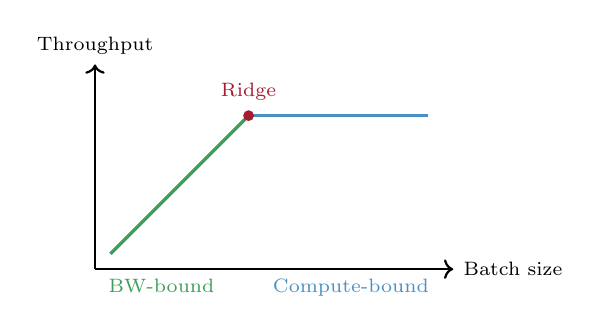
\begin{tikzpicture}[scale=0.65]
  \draw[->, thick] (0,0) -- (7,0) node[right, font=\scriptsize] {Batch size};
  \draw[->, thick] (0,0) -- (0,4) node[above, font=\scriptsize] {Throughput};
  \draw[very thick, datastroke] (0.3,0.3) -- (3,3);
  \draw[very thick, computestroke] (3,3) -- (6.5,3);
  \fill[crimson] (3,3) circle (3pt);
  \node[above, font=\scriptsize, crimson] at (3,3.1) {Ridge};
  \node[below, font=\scriptsize, datastroke] at (1.3,0) {BW-bound};
  \node[below, font=\scriptsize, computestroke] at (5,0) {Compute-bound};
\end{tikzpicture}
\end{frame}

% --- Slide 1.11: Live Demo --- Batch Size Sweep ---
\begin{frame}[fragile]{Live Demo: Finding the Ridge Point}
\note{[3 min] Run this loop live. Show how the bottleneck flips
from Memory to Compute as batch size increases.
Before running, ask: ``At what batch size do you
predict the bottleneck will flip?'' Take guesses.
% -- FLEX: [CORE]
}

\small
\begin{lstlisting}
llama = mlsysim.Models.Language.Llama3_8B
hw    = mlsysim.Hardware.Cloud.H100

for bs in [1, 4, 16, 64, 128, 256]:
    p = mlsysim.Engine.solve(llama, hw, batch_size=bs)
    print(f"bs={bs:>3d}  {p.bottleneck:<8s}  "
          f"MFU={p.mfu:.3f}")
\end{lstlisting}

\vspace{0.3cm}
\begin{exampleblock}{What to observe}
  \begin{itemize}
    \item Bottleneck flips from \texttt{Memory} to \texttt{Compute}
    \item MFU climbs as batch size increases (better hardware utilization)
    \item Latency grows but throughput (tokens/s) improves
  \end{itemize}
\end{exampleblock}
\end{frame}

% --- Slide 1.12: Exercise 1 ---
\begin{frame}[fragile]{Exercise 1: Find the Crossover}
\note{[5 min] Attendees work individually.
At what batch size does Llama-3 8B on H100 transition
from memory-bound to compute-bound?
Expected: around bs=32--64 depending on precision.
Turn to your neighbor: did you get the same answer? Why or why not? 60 seconds.
% -- FLEX: [CORE] --- this is a critical hands-on moment.
}

\centering
\Large\bfseries
Hands-On Exercise\\[0.5cm]
\normalsize

\textbf{Question:} At what batch size does Llama-3 8B on H100
transition from memory-bound to compute-bound?

\vspace{0.3cm}
\begin{lstlisting}
for bs in range(1, 129):
    p = mlsysim.Engine.solve(llama, hw, batch_size=bs)
    if p.bottleneck == "Compute":
        print(f"Crossover at batch size {bs}")
        break
\end{lstlisting}

\vspace{0.3cm}
\textit{Bonus: Try the same on A100. Does the crossover happen
at the same batch size? Why or why not?}
\end{frame}

% --- Slide 1.13: The Ridge Point Explained ---
\begin{frame}{The Ridge Point: Hardware DNA}
\note{[2 min] ``The ridge point is a property of the hardware,
not the workload. It tells you how many FLOPs per byte the chip
can sustain before compute becomes the ceiling.''
% -- FLEX: [CORE]
}

\small
\[
  \text{Ridge Point} = \frac{\text{Peak FLOPS}}{\text{Peak BW}}
  \;\;\bigl[\text{FLOP/byte}\bigr]
\]

\vspace{0.2cm}
\scriptsize
\begin{tabular}{llccc}
\toprule
\textbf{Vendor} & \textbf{Hardware} & \textbf{Peak FP16} & \textbf{HBM BW} & \textbf{Ridge} \\
\midrule
NVIDIA & H100 SXM  & 989 TFLOPS  & 3.35 TB/s & 295 FLOP/B \\
NVIDIA & B200      & 2.25 PFLOPS & 8.0 TB/s  & 281 FLOP/B \\
AMD    & MI300X    & 1,307 TFLOPS & 5.3 TB/s & 247 FLOP/B \\
Intel  & Gaudi\,3  & 1,835 TFLOPS & 3.7 TB/s & 496 FLOP/B \\
\bottomrule
\end{tabular}
\small

\vspace{0.3cm}
\begin{itemize}
  \item Higher ridge $\Rightarrow$ more workloads are memory-bound on this chip
  \item \alert{FLOPS grow faster than bandwidth across GPU generations}
  \item The memory wall is getting \textbf{worse}, not better
\end{itemize}
\end{frame}

% --- Slide 1.14: Predict Before You Peek #2 ---
\begin{frame}{Predict: ResNet-50 vs Llama-3 8B}
\note{[2 min] ``ResNet-50 at batch 256 vs Llama-3 8B at batch 1.
Which is compute-bound and which is memory-bound?''
Give 30 seconds. Expected: ResNet at high batch is compute-bound;
Llama at bs=1 is memory-bound.
Turn to your neighbor: did you get the same answer? Why or why not? 60 seconds.
% -- FLEX: [CORE]
}

\centering
\Large\bfseries
Two workloads on the same H100.\\[0.3cm]
\normalsize
Which is compute-bound? Which is memory-bound?\\[0.5cm]

\pause

\small
\begin{tabular}{lcc}
\toprule
              & \textbf{ResNet-50 (bs=256)} & \textbf{Llama-3 8B (bs=1)} \\
\midrule
Total FLOPs   & $2.05 \times 10^{12}$       & $1.6 \times 10^{10}$ \\
Weight bytes   & 50 MB (FP16)               & 16 GB (FP16) \\
AI (FLOP/B)   & $\sim$41{,}000              & $\sim$1 \\
\midrule
\textbf{Regime} & \colorbox{computeblue}{Compute-bound} & \colorbox{datagreen}{Memory-bound} \\
\bottomrule
\end{tabular}

\vspace{0.3cm}
\pause
\alert{Same hardware, completely different bottlenecks.}\\
\textit{The workload determines the regime, not the GPU.}
\end{frame}

% --- Slide 1.15: Key Takeaway (Part 1) ---
\begin{frame}{Part 1: Key Takeaway}
\note{[1 min] Summarize in one sentence. Repeat it twice.
``The bottleneck determines the speedup. Know your regime.''
% -- FLEX: [CORE]
}

\centering\Large

\textbf{The bottleneck determines the speedup.}\\[0.5cm]

\normalsize
\begin{itemize}
  \item The Roofline model tells you \textit{which} constraint is binding.
  \item Batch size is the primary knob that moves you between regimes.
  \item More FLOPS only helps if you are compute-bound.
  \item More bandwidth only helps if you are memory-bound.
  \item \texttt{Engine.solve()} answers this in one line.
\end{itemize}
\end{frame}

% --- Roadmap: After Break ---
\begin{frame}{Roadmap: You Are Here}
\note{[1 min] Quick orientation after break. We now move from single-op analysis to serving.}

\centering\small
\begin{tabular}{rll}
\toprule
\textbf{Time} & \textbf{Part} & \textbf{Status} \\
\midrule
9:00--9:30   & Part 0: Welcome \& Setup     & \checkmark \\
9:30--10:30  & Part 1: Iron Law \& Roofline  & \checkmark \\
\rowcolor{crimson!12}
10:45--11:45 & \textbf{Part 2: Memory Walls \& Serving} & \textbf{$\leftarrow$ You are here} \\
11:45--12:00 & Part 3: Compression & \\
\bottomrule
\end{tabular}
\end{frame}

% =============================================================================
% PART 2: MEMORY WALLS & SERVING (12 slides)
% =============================================================================
\section{Memory Walls \& Serving}

% --- Slide 2.1: Key Question ---
\begin{frame}{Key Question}
\note{[1 min] ``You have seen that LLM inference at batch 1 is
memory-bound. But serving is more complex than a single forward
pass. What makes LLM serving fundamentally different from
CNN inference?''
% -- FLEX: [CORE]
}

\centering
\Large\bfseries
Why does the first token take 50\,ms\\[0.2cm]
but each next token only takes 5\,ms?
\end{frame}

% --- Slide 2.2: Two Phases of LLM Serving ---
\begin{frame}{Wall 4: Prefill vs Decode --- Two Different Physics}
\note{[3 min] ``Prefill is like reading a book fast (compute-intensive).
Decode is like looking up one word at a time in a dictionary
(memory-intensive). Same model, different bottlenecks.''
% -- FLEX: [CORE]
}

\small
\wallbox{The Serving Wall}{
\begin{tabular}{lcl}
  \textbf{TTFT} (Prefill) & $=$ & $\dfrac{\text{Prefill FLOPs}}{\text{Peak FLOPS} \times \text{MFU}}$
  \quad\colorbox{computeblue}{Compute-bound} \\[10pt]
  \textbf{ITL} (Decode)   & $=$ & $\dfrac{\text{Weight Bytes}}{\text{Bandwidth}}$
  \quad\colorbox{datagreen}{Memory-bound}
\end{tabular}
}

\vspace{0.3cm}
\begin{columns}[T]
\begin{column}{0.48\textwidth}
\textbf{Prefill} (process the prompt)
\begin{itemize}\setlength\itemsep{2pt}
  \item All prompt tokens in parallel
  \item $O(S^2)$ attention + $O(S \cdot P)$ linear
  \item Compute-bound (high AI)
  \item Determines \textbf{TTFT}
\end{itemize}
\end{column}
\begin{column}{0.48\textwidth}
\textbf{Decode} (generate tokens)
\begin{itemize}\setlength\itemsep{2pt}
  \item One token at a time
  \item Must reload all weights per token
  \item Memory-bound (AI $\approx$ 1)
  \item Determines \textbf{ITL}
\end{itemize}
\end{column}
\end{columns}
\end{frame}

% --- Slide 2.3: KV Cache --- The Hidden Consumer ---
\begin{frame}{Wall 5: The KV Cache --- Hidden Memory Consumer}
\note{[3 min] ``Each active request carries its own memory of the
conversation.'' Quick math: how much KV cache does one Llama-3 8B
request at 4K context need in FP16?
Expected: 2 * 32 * 32 * 128 * 4096 * 2 bytes = ~2 GB.
% -- FLEX: [CORE]
}

\small
\wallbox{The Batching Wall}{
\[
  \text{KV cache} = 2 \times L \times H \times d \times S \times B \times \text{bpp}
\]
}

\vspace{0.2cm}
\textbf{Llama-3 8B at 4K context, FP16:}
\begin{itemize}
  \item $2 \times 32 \times 32 \times 128 \times 4096 \times 2\;\text{bytes} \approx 2\;\text{GB}$ per request
  \item H100 has 80 GB HBM --- model weights take 16 GB
  \item Remaining 64 GB $\div$ 2 GB/request $=$ \textbf{$\sim$32 concurrent requests}
\end{itemize}

\vspace{0.2cm}
\begin{alertblock}{The serving paradox}
  You want high batch size (for throughput) but KV cache limits how
  many requests fit in memory. \alert{Memory capacity, not compute, limits concurrency.}
\end{alertblock}
\end{frame}

% --- Slide 2.4: Live Demo --- ServingModel ---
\begin{frame}[fragile]{Live Demo: Two-Phase Serving Analysis}
\note{[2 min] Run ServingModel live. Point out TTFT vs ITL in output.
Show that TTFT is compute-bound and ITL is memory-bound.
% -- FLEX: [CORE]
}

\small
\begin{lstlisting}
serving = mlsysim.ServingModel()
result  = serving.solve(llama, hw,
                        seq_len=4096, batch_size=1)
print(f"TTFT: {result.ttft:~P}")
print(f"ITL:  {result.itl:~P}")
print(f"KV cache/req: {result.kv_cache_per_request:~P}")
\end{lstlisting}

\vspace{0.2cm}
\begin{exampleblock}{Expected output}
  TTFT $\approx$ 20--50 ms (compute-bound),
  ITL $\approx$ 5 ms (memory-bound),
  KV cache per request $\approx$ 2 GB
\end{exampleblock}
\end{frame}

% --- Slide 2.5: Continuous Batching ---
\begin{frame}{Continuous Batching: Don't Wait, Serve}
\note{[2 min] ``In static batching, the GPU waits for the longest
request to finish. In continuous batching, new requests start
as soon as any slot frees up. Throughput can improve 2--5x.''
% -- FLEX: [OPTIONAL] Can summarize quickly if behind schedule.
}

\small
\begin{columns}[T]
\begin{column}{0.48\textwidth}
\textbf{Static batching}
\begin{itemize}\setlength\itemsep{2pt}
  \item Pad all sequences to max length
  \item GPU idle while short requests finish
  \item Throughput limited by longest request
  \item Simple to implement
\end{itemize}
\end{column}
\begin{column}{0.48\textwidth}
\textbf{Continuous batching}
\begin{itemize}\setlength\itemsep{2pt}
  \item Insert new requests per iteration
  \item No padding waste
  \item Throughput 2--5$\times$ higher
  \item Used by vLLM, TGI, TensorRT-LLM
\end{itemize}
\end{column}
\end{columns}

\vspace{0.3cm}
\centering
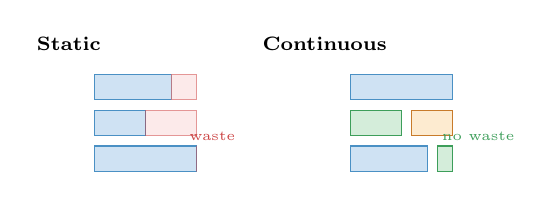
\begin{tikzpicture}[scale=0.65, >=Stealth]
  % Static
  \node[font=\scriptsize\bfseries] at (0, 2.5) {Static};
  \foreach \i/\len in {0/4, 1/2, 2/3} {
    \fill[computeblue, draw=computestroke] (0.5, \i*0.7) rectangle ({0.5 + \len*0.5}, \i*0.7+0.5);
    \fill[errorfill, draw=errorstroke, opacity=0.5] ({0.5 + \len*0.5}, \i*0.7) rectangle (2.5, \i*0.7+0.5);
  }
  \node[font=\tiny, errorstroke] at (2.8, 0.7) {waste};

  % Continuous
  \node[font=\scriptsize\bfseries] at (5, 2.5) {Continuous};
  \fill[computeblue, draw=computestroke] (5.5, 1.4) rectangle (7.5, 1.9);
  \fill[datagreen, draw=datastroke] (5.5, 0.7) rectangle (6.5, 1.2);
  \fill[routingorange, draw=routingstroke] (6.7, 0.7) rectangle (7.5, 1.2);
  \fill[computeblue, draw=computestroke] (5.5, 0) rectangle (7, 0.5);
  \fill[datagreen, draw=datastroke] (7.2, 0) rectangle (7.5, 0.5);
  \node[font=\tiny, datastroke] at (8, 0.7) {no waste};
\end{tikzpicture}
\end{frame}

% --- Slide 2.6: PagedAttention ---
\begin{frame}[fragile]{PagedAttention: Virtual Memory for KV Cache}
\note{[2 min] ``Just like OS virtual memory pages physical RAM,
PagedAttention pages the KV cache. Non-contiguous blocks mean
no fragmentation, so you can fit more requests.''
% -- FLEX: [OPTIONAL]
}

\small
\textbf{The problem:} Pre-allocated KV cache wastes memory on short sequences.

\textbf{The solution} (Kwon et al., 2023 --- vLLM):
\begin{itemize}
  \item Divide KV cache into fixed-size \textbf{pages} (e.g., 16 tokens each)
  \item Allocate pages on demand, not up front
  \item Non-contiguous storage eliminates fragmentation
  \item Memory utilization improves from $\sim$50\% to $>$95\%
\end{itemize}

\vspace{0.2cm}
\begin{exampleblock}{Impact}
  With the same 80 GB H100, PagedAttention can serve
  \textbf{2--4$\times$ more concurrent requests} than static allocation.
\end{exampleblock}

\vspace{0.2cm}
\begin{lstlisting}
# mlsysim models this with ContinuousBatchingModel
cb = mlsysim.ContinuousBatchingModel()
result = cb.solve(model, hw, seq_len=4096,
                  max_batch_size=32, page_size=16)
print(f"Max concurrent: {result.max_concurrent_requests}")
\end{lstlisting}
\end{frame}

% --- Slide 2.7: Predict Before You Peek #3 ---
\begin{frame}{Predict: How Many Concurrent Requests?}
\note{[2 min] Predict-before-reveal. Give 60 seconds.
H100 80 GB, Llama-3 8B FP16, 4K context. How many concurrent requests?
Expected: weights = 16 GB, remaining = 64 GB.
PagedAttention (95\% util): ~30. Without (50\% util): ~16.
Turn to your neighbor: did you get the same answer? Why or why not? 60 seconds.
% -- FLEX: [CORE]
}

\centering
\Large\bfseries
H100 (80 GB), Llama-3 8B (FP16), 4K context.\\[0.5cm]
\normalsize
How many concurrent requests can you serve?\\[0.3cm]

\pause

\small
\begin{tabular}{lcc}
\toprule
  & \textbf{Static alloc.} & \textbf{PagedAttention} \\
\midrule
KV cache utilization & $\sim$50\% & $\sim$95\% \\
Effective memory/req & $\sim$4 GB & $\sim$2.1 GB \\
Max concurrent & $\sim$16 & $\sim$30 \\
\bottomrule
\end{tabular}

\vspace{0.3cm}
\pause
\alert{PagedAttention nearly doubles serving capacity without changing hardware.}
\end{frame}

% --- Slide 2.8: Speculative Decoding ---
\begin{frame}[fragile]{Speculative Decoding: Betting on the Draft}
\note{[2 min] ``Use a small draft model to guess the next K tokens.
Then verify all K in a single forward pass of the big model.
If the draft is right 70\% of the time and K=5, you effectively
decode ~3.5 tokens per forward pass instead of 1.''
% -- FLEX: [OPTIONAL]
}

\small
\textbf{Insight:} Decode is memory-bound $\Rightarrow$ the GPU has spare compute.

\textbf{Speculative decoding} (Leviathan et al., 2023):
\begin{enumerate}\setlength\itemsep{2pt}
  \item \textbf{Draft} $K$ tokens with a small model (fast, low quality)
  \item \textbf{Verify} all $K$ tokens in one forward pass of the big model
  \item \textbf{Accept} the longest prefix that matches
  \item Speedup $\approx K \times \alpha$ where $\alpha$ is acceptance rate
\end{enumerate}

\vspace{0.2cm}
\begin{lstlisting}
# mlsysim supports speculative decoding
draft = mlsysim.Models.Language.Llama3_8B  # smaller
result = serving.solve(model, hw, seq_len=4096,
          draft_model=draft, draft_acceptance_rate=0.7)
print(f"Speedup: {result.speculative_speedup:.2f}x")
\end{lstlisting}
\end{frame}

% --- Slide 2.9: Disaggregated Serving ---
\begin{frame}[fragile]{Disaggregated Serving: Right Hardware for Each Phase}
\note{[2 min] ``Split prefill and decode onto different node types.
Prefill nodes optimize for FLOPS, decode nodes optimize for
bandwidth. Transfer KV cache over the network between them.''
% -- FLEX: [OPTIONAL]
}

\small
\textbf{Key insight:} Prefill and decode have \textit{opposite} hardware preferences.

\begin{columns}[T]
\begin{column}{0.48\textwidth}
\textbf{Prefill node}
\begin{itemize}\setlength\itemsep{2pt}
  \item Needs high FLOPS
  \item Moderate memory
  \item E.g., H100 at high utilization
\end{itemize}
\end{column}
\begin{column}{0.48\textwidth}
\textbf{Decode node}
\begin{itemize}\setlength\itemsep{2pt}
  \item Needs high BW
  \item Large memory (for KV cache)
  \item E.g., many smaller accelerators
\end{itemize}
\end{column}
\end{columns}

\vspace{0.3cm}
\begin{lstlisting}
# Disaggregated serving in mlsysim
result = serving.solve(model, hw, seq_len=4096,
          decode_hardware=mlsysim.Hardware.Cloud.A100)
print(f"TTFT: {result.ttft:~P}  ITL: {result.itl:~P}")
\end{lstlisting}

\vspace{0.2cm}
\alert{Trade-off: network transfer of KV cache adds latency between phases.}
\end{frame}

% --- Slide 2.10: Exercise 2 ---
\begin{frame}[fragile]{Exercise 2: Serving Capacity Planning}
\note{[5 min] Attendees work in pairs.
How many concurrent Llama-3 8B requests (4K context) can an H100
serve while maintaining ITL < 10ms?
Expected: ~30 with PagedAttention at FP16. Binding: memory capacity.
Turn to your neighbor: did you get the same answer? Why or why not? 60 seconds.
% -- FLEX: [CORE]
}

\centering
\Large\bfseries
Hands-On Exercise\\[0.5cm]
\normalsize

\textbf{Question:} You run Llama-3 8B (FP16) on one H100 with 4K context.\\
Your SLA requires ITL $<$ 10 ms.\\
How many concurrent requests can you serve?

\vspace{0.3cm}
\begin{lstlisting}
cb = mlsysim.ContinuousBatchingModel()
result = cb.solve(llama, hw, seq_len=4096,
                  max_batch_size=64, page_size=16)
print(f"Max concurrent: {result.max_concurrent_requests}")
\end{lstlisting}

\vspace{0.2cm}
\textit{Bonus: What happens if you switch to INT8 precision?
Does concurrency double?}
\end{frame}

% --- Slide 2.11: Fallacies ---
\begin{frame}{Fallacies: Serving Edition}
\note{[2 min] Walk through each fallacy with the quantitative
counter-evidence.
% -- FLEX: [OPTIONAL] --- can trim to 2 fallacies if behind.
}

\small
\textbf{Fallacy:} \textit{``Faster GPUs always reduce latency.''}\\
A 3.2$\times$ FLOPS improvement (A100 $\to$ H100) yields only
1.7$\times$ ITL improvement because decode is memory-bound.

\vspace{0.3cm}
\textbf{Fallacy:} \textit{``Doubling memory doubles serving capacity.''}\\
Weights are fixed overhead. Going from 80 GB to 160 GB adds 80 GB,
but KV cache per request stays $\sim$2 GB. Capacity goes from $\sim$32
to $\sim$72 ($\sim$2.3$\times$), not 2$\times$.

\vspace{0.3cm}
\textbf{Fallacy:} \textit{``Batch size 1 is fine for LLM inference.''}\\
At bs=1, MFU $<$ 5\%. You are paying for 989 TFLOPS and using $<$ 50.
Continuous batching can recover 10--20$\times$ throughput.
\end{frame}

% --- Slide 2.12: Part 2 Key Takeaway ---
\begin{frame}{Part 2: Key Takeaway}
\note{[1 min] One sentence summary, repeat twice.
% -- FLEX: [CORE]
}

\centering\Large

\textbf{LLM serving has two phases\\with opposite bottlenecks.}\\[0.5cm]

\normalsize
\begin{itemize}
  \item \textbf{Prefill} (TTFT) is compute-bound --- optimize with parallelism.
  \item \textbf{Decode} (ITL) is memory-bound --- optimize with bandwidth.
  \item \textbf{KV cache} limits concurrency --- optimize with PagedAttention.
  \item \texttt{ServingModel.solve()} decomposes both phases in one call.
\end{itemize}
\end{frame}

% =============================================================================
% PART 3: COMPRESSION & EFFICIENCY (8 slides)
% =============================================================================
\section{Compression \& Efficiency}

% --- Slide 3.1: Key Question ---
\begin{frame}{Key Question}
\note{[1 min] ``If we can shrink the model, we move less data,
and the memory wall recedes. But there is a catch.''
% -- FLEX: [CORE]
}

\centering
\Large\bfseries
Can you make the model 4$\times$ smaller\\[0.2cm]
and get a 4$\times$ speedup?
\end{frame}

% --- Slide 3.2: Wall 13 --- Compression ---
\begin{frame}{Wall 13: The Fidelity Wall}
\note{[2 min] ``Storage always shrinks. But inference speedup
depends on the method. This distinction trips up everyone.''
% -- FLEX: [CORE]
}

\small
\wallbox{The Fidelity Wall}{
\[
  \text{Compression}_{\text{quant}} = \frac{32}{\text{bits}},
  \qquad
  \text{Compression}_{\text{prune}} = \frac{1}{1 - \text{sparsity}}
\]
}

\vspace{0.3cm}
\begin{tabular}{lccc}
\toprule
\textbf{Method} & \textbf{Storage} & \textbf{Speedup} & \textbf{Accuracy} \\
\midrule
FP32 $\to$ FP16 & 2$\times$ & 2$\times$ & $\sim$0\% loss \\
FP16 $\to$ INT8  & 2$\times$ & 1.5--2$\times$ & $<$1\% loss \\
FP16 $\to$ INT4  & 4$\times$ & 2--3$\times$ & 2--5\% loss \\
50\% unstructured prune & 2$\times$ & \alert{1$\times$ (no speedup!)} & 1--3\% loss \\
50\% structured prune & 2$\times$ & $\sim$2$\times$ & 2--5\% loss \\
2:4 N:M sparsity & 2$\times$ & 2$\times$ & 1--2\% loss \\
\bottomrule
\end{tabular}

\vspace{0.2cm}
\alert{Unstructured pruning saves storage but gives zero GPU speedup.\\
Only structured patterns accelerate hardware execution.}
\end{frame}

% --- Slide 3.3: Quantization Deep Dive ---
\begin{frame}{Quantization: Trading Bits for Speed}
\note{[2 min] Walk through the precision ladder.
``If you quantize Llama-3 8B from FP16 to INT4, how much memory?''
Expected: 8B * 0.5 bytes = 4 GB. Down from 16 GB.
% -- FLEX: [CORE]
}

\small
\begin{columns}[T]
\begin{column}{0.55\textwidth}
\textbf{The precision ladder:}

\vspace{0.2cm}
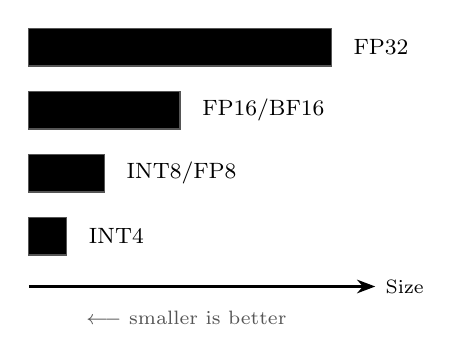
\begin{tikzpicture}[scale=0.8, >=Stealth]
  \foreach \i/\label/\bits/\color in {
    0/FP32/32/errorfill,
    1/FP16\slash BF16/16/routingorange,
    2/INT8\slash FP8/8/computeblue,
    3/INT4/4/datagreen} {
    \fill[\color, draw=midgray] (0, 3-\i) rectangle ({0.15*\bits}, 3.6-\i);
    \node[right, font=\footnotesize] at ({0.15*\bits + 0.2}, 3.3-\i) {\label};
  }
  \draw[->, thick] (0, -0.5) -- (5.5, -0.5) node[right, font=\scriptsize] {Size};
  \node[font=\scriptsize, midgray] at (2.5, -1) {$\longleftarrow$ smaller is better};
\end{tikzpicture}
\end{column}
\begin{column}{0.42\textwidth}
\textbf{Llama-3 8B memory:}
\scriptsize
\begin{tabular}{lc}
\toprule
Precision & Weight Size \\
\midrule
FP32 & 32 GB \\
FP16 & 16 GB \\
INT8 & 8 GB \\
INT4 & 4 GB \\
\bottomrule
\end{tabular}

\vspace{0.3cm}
\normalsize
At INT4, Llama-3 8B fits in\\
a \textbf{laptop GPU} (6 GB).
\end{column}
\end{columns}
\end{frame}

% --- Slide 3.4: Live Demo --- CompressionModel ---
\begin{frame}[fragile]{Live Demo: Quantization Impact}
\note{[2 min] Run CompressionModel live. Show storage savings
and speedup side by side.
% -- FLEX: [CORE]
}

\small
\begin{lstlisting}
comp = mlsysim.CompressionModel()
for bits in [16, 8, 4]:
    r = comp.solve(llama, hw, method="quantization",
                   target_bitwidth=bits)
    print(f"INT{bits}: size={r.compressed_size:~P}  "
          f"speedup={r.inference_speedup:.1f}x")
\end{lstlisting}

\vspace{0.2cm}
\begin{exampleblock}{What to observe}
  \begin{itemize}
    \item Storage shrinks linearly with bit reduction
    \item Speedup follows storage for quantization (structured by nature)
    \item Accuracy degrades modestly at INT8, more at INT4
  \end{itemize}
\end{exampleblock}
\end{frame}

% --- Slide 3.5: Structured vs Unstructured Pruning ---
\begin{frame}[fragile]{Pruning: The Structure Matters}
\note{[2 min] ``Unstructured pruning zeros out individual weights.
The matrix is still the same shape, so the GPU does the same
number of operations. No speedup! Structured pruning removes
entire rows/columns, physically shrinking the matrix.''
WARN: Students assume any compression = speedup.
% -- FLEX: [CORE]
}

\small
\begin{columns}[T]
\begin{column}{0.48\textwidth}
\textbf{Unstructured}
\begin{itemize}\setlength\itemsep{2pt}
  \item Zero out individual weights
  \item Matrix shape unchanged
  \item GPU does same work (skip zeros? nope)
  \item \alert{Storage savings only}
\end{itemize}
\end{column}
\begin{column}{0.48\textwidth}
\textbf{Structured / N:M}
\begin{itemize}\setlength\itemsep{2pt}
  \item Remove entire rows/columns, or\\
        2:4 pattern (Ampere+)
  \item Physically smaller matrices
  \item GPU hardware support (2:4 $\to$ 2$\times$)
  \item \textbf{Real speedup}
\end{itemize}
\end{column}
\end{columns}

\vspace{0.3cm}
\begin{lstlisting}
for stype in ["unstructured", "structured", "n_m"]:
    r = comp.solve(llama, hw, method="pruning",
            sparsity=0.5, sparsity_type=stype)
    print(f"{stype:>14}: {r.inference_speedup:.1f}x")
\end{lstlisting}
\end{frame}

% --- Slide 3.5b: Predict --- What Does INT4 Change? ---
\begin{frame}{Predict: What Does INT4 Change?}
\note{[1 min] Quick poll. Most say "latency gets better." The real answer is fleet size.
Turn to your neighbor: did you get the same answer? Why or why not? 60 seconds.}
\centering
\Large
\textbf{You quantize Llama-3 70B from FP16 to INT4.}\\[0.5cm]
\normalsize
What is the BIGGEST impact on your serving infrastructure?\\[0.3cm]
\begin{enumerate}[(A)]
  \item Inference latency drops by 4$\times$
  \item Model quality degrades significantly
  \item \textbf{You need half as many GPUs}
  \item Memory bandwidth becomes the bottleneck
\end{enumerate}
\end{frame}

% --- Slide 3.6: Predict Before You Peek #4 ---
\begin{frame}{Predict: INT4 Llama-3 8B on H100}
\note{[2 min] Predict-before-reveal. If you quantize to INT4 at bs=1,
is it still memory-bound? Yes! Load time = 4/3350 = 1.2 ms.
Compute still ~0.03 ms. Still memory-bound but 4x faster.
Turn to your neighbor: did you get the same answer? Why or why not? 60 seconds.
% -- FLEX: [CORE]
}

\centering
\Large\bfseries
Quantize Llama-3 8B to INT4.\\
Run inference at batch size 1 on H100.\\[0.5cm]
\normalsize
Is it still memory-bound?\\[0.3cm]

\pause

\small
\begin{tabular}{lcc}
\toprule
              & \textbf{FP16} & \textbf{INT4} \\
\midrule
Weight size   & 16 GB & 4 GB \\
Load time     & 4.8 ms & 1.2 ms \\
Compute time  & 0.03 ms & 0.03 ms \\
\midrule
Bottleneck    & Memory & \textbf{Still Memory!} \\
Decode speedup & --- & \textbf{4$\times$} \\
\bottomrule
\end{tabular}

\vspace{0.3cm}
\pause
\alert{INT4 gives 4$\times$ faster decode, but the GPU is still memory-bound.\\
The memory wall is that deep.}
\end{frame}

% --- Slide 3.7: Exercise 3 ---
\begin{frame}[fragile]{Exercise 3: Compression Tradeoffs}
\note{[5 min] Compare INT8 quantization vs 50\% structured pruning
for Llama-3 8B on H100. Which gives better speedup per accuracy loss?
Expected: INT8 wins (~2x speedup, <1\% loss vs 2-5\% loss).
Turn to your neighbor: did you get the same answer? Why or why not? 60 seconds.
% -- FLEX: [CORE]
}

\centering
\Large\bfseries
Hands-On Exercise\\[0.5cm]
\normalsize

\textbf{Question:} For Llama-3 8B on H100, which is the better deal?
\begin{enumerate}
  \item INT8 quantization
  \item 50\% structured pruning
\end{enumerate}
Compare speedup per accuracy point lost.

\vspace{0.3cm}
\begin{lstlisting}
r1 = comp.solve(llama, hw, method="quantization",
                target_bitwidth=8)
r2 = comp.solve(llama, hw, method="pruning",
        sparsity=0.5, sparsity_type="structured")
print(f"Quant: {r1.inference_speedup:.1f}x / "
      f"{abs(r1.accuracy_delta):.1%} loss")
print(f"Prune: {r2.inference_speedup:.1f}x / "
      f"{abs(r2.accuracy_delta):.1%} loss")
\end{lstlisting}
\end{frame}

% --- Slide 3.7b: Compression Changes Fleet Architecture ---
\begin{frame}{Compression Changes Fleet Architecture}
\note{[3 min] This is the ``aha'' that compression is architecture, not optimization.
The punchline: INT4 halves your GPU count AND your electricity bill.}

\small
\textbf{Llama-3 70B Serving Fleet:}

\vspace{0.3cm}
\begin{tabular}{@{}lrrr@{}}
\toprule
Precision & Model Size & GPUs Needed & Annual Cost \\
\midrule
FP16 & 140 GB & 4 (TP=4) & \$480K \\
INT8 & 70 GB & 2 (TP=2) & \$240K \\
INT4 & 35 GB & 1 & \$120K \\
\bottomrule
\end{tabular}

\vspace{0.3cm}
\textbf{INT4 doesn't just improve latency --- it eliminates 3 GPUs per replica.}\\
At 100 replicas for 1000 QPS: that's \textbf{300 fewer GPUs} and \textbf{\$36M saved per year}.

\vfill
\centering
\small\textcolor{gray}{This is why quantization is a Day 1 architectural decision, not a Day 100 optimization.}
\end{frame}

% --- Slide 3.8: Part 3 Key Takeaway ---
\begin{frame}{Part 3: Key Takeaway}
\note{[1 min] One sentence. Repeat.
% -- FLEX: [CORE]
}

\centering\Large

\textbf{Storage savings $\neq$ inference speedup.}\\[0.5cm]

\normalsize
\begin{itemize}
  \item Quantization gives both storage and speed gains.
  \item Unstructured pruning gives storage only --- zero GPU speedup.
  \item N:M sparsity (2:4) is the hardware-friendly middle ground.
  \item Even at INT4, LLM decode is \textit{still} memory-bound.
  \item \texttt{CompressionModel.solve()} quantifies the full tradeoff.
\end{itemize}
\end{frame}

% --- Roadmap: After Lunch ---
\begin{frame}{Roadmap: Afternoon Session}
\note{[1 min] Re-energize the room. ``Welcome back. The morning was about
single-node physics. The afternoon is about fleets, money, and carbon.''}

\centering\small
\begin{tabular}{rll}
\toprule
\textbf{Time} & \textbf{Part} & \textbf{Status} \\
\midrule
9:00--12:00  & Parts 0--3: Single Node   & \checkmark Done \\
\midrule
\rowcolor{crimson!12}
1:00--2:15   & \textbf{Part 4: Going Distributed} & \textbf{$\leftarrow$ You are here} \\
2:30--3:15   & Part 5: Economics \& Sustainability & \\
3:15--3:45   & Part 6: Design Space Exploration & \\
3:45--4:15   & Part 7: TinyML to Frontier & \\
4:15--4:45   & Part 8: Advanced Topics & \\
4:45--5:00   & Part 9: Wrap-Up \& Capstone & \\
\bottomrule
\end{tabular}
\end{frame}

% =============================================================================
% PART 4: GOING DISTRIBUTED (15 slides)
% =============================================================================
\section{Going Distributed}

% --- Slide 4.1: Key Question ---
\begin{frame}{Key Question}
\note{[1 min] ``Your model does not fit on one GPU. Or it fits but
training would take a year. Either way, you need more GPUs.
But adding GPUs is not free.''
% -- FLEX: [CORE]
}

\centering
\Large\bfseries
If 1 GPU takes 30 days,\\[0.2cm]
do 1000 GPUs take 43 minutes?
\end{frame}

% --- Slide 4.2: Why Distribute? ---
\begin{frame}{Why Distribute?}
\note{[2 min] ``Two reasons to go distributed: (1) the model does not
fit in one GPU's memory, or (2) you want to finish sooner.
Reason 1 is a hard constraint. Reason 2 is an optimization.''
% -- FLEX: [CORE]
}

\small
\textbf{Reason 1: Model does not fit}
\begin{itemize}
  \item Llama-3 70B FP16 $=$ 140 GB $>$ H100's 80 GB
  \item \alert{Must} split across at least 2 GPUs
\end{itemize}

\vspace{0.3cm}
\textbf{Reason 2: Time-to-train}
\begin{itemize}
  \item 1 H100 training Llama-3 70B $\approx$ 15 GPU-years
  \item 1024 H100s $\approx$ 5 days (if scaling were perfect)
  \item But scaling is \textit{never} perfect...
\end{itemize}

\vspace{0.3cm}
\centering
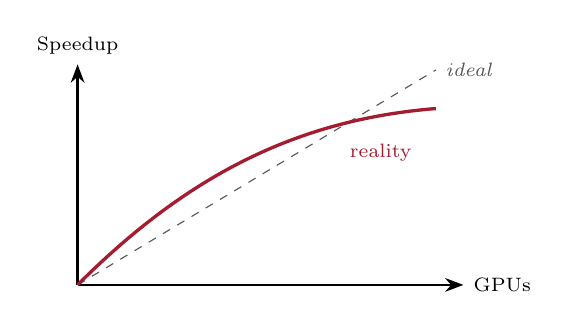
\begin{tikzpicture}[scale=0.7, >=Stealth]
  \draw[->, thick] (0,0) -- (7,0) node[right, font=\scriptsize] {GPUs};
  \draw[->, thick] (0,0) -- (0,4) node[above, font=\scriptsize] {Speedup};
  \draw[dashed, midgray] (0,0) -- (6.5,3.9) node[right, font=\scriptsize\itshape] {ideal};
  \draw[very thick, crimson] (0,0) .. controls (2,2) and (4,3) .. (6.5,3.2);
  \node[font=\scriptsize, crimson] at (5.5, 2.4) {reality};
\end{tikzpicture}
\end{frame}

% --- Slide 4.3: The Three Dimensions of Parallelism ---
\begin{frame}{3D Parallelism: DP $\times$ TP $\times$ PP}
\note{[3 min] ``Every distributed strategy is a combination of three
dimensions.'' WARN: Students often confuse TP and PP.
TP splits within a layer; PP splits between layers.
% -- FLEX: [CORE]
}

\small
\begin{columns}[T]
\begin{column}{0.32\textwidth}
\textbf{Data Parallel (DP)}
\begin{itemize}\setlength\itemsep{1pt}\footnotesize
  \item Replicate full model
  \item Split data across replicas
  \item AllReduce gradients
  \item \textit{Most common}
\end{itemize}
\end{column}
\begin{column}{0.32\textwidth}
\textbf{Tensor Parallel (TP)}
\begin{itemize}\setlength\itemsep{1pt}\footnotesize
  \item Split each layer's weights
  \item Split activations, not data
  \item AllReduce per layer (2$\times$!)
  \item Needs fast interconnect
\end{itemize}
\end{column}
\begin{column}{0.32\textwidth}
\textbf{Pipeline Parallel (PP)}
\begin{itemize}\setlength\itemsep{1pt}\footnotesize
  \item Split model into stages
  \item Each GPU owns $L/\text{PP}$ layers
  \item Pipeline bubbles
  \item Needs less bandwidth
\end{itemize}
\end{column}
\end{columns}

\vspace{0.3cm}
Total GPUs: $N = \text{DP} \times \text{TP} \times \text{PP}$

\vspace{0.2cm}
\centering
\scriptsize
\begin{tabular}{lccc}
\toprule
\textbf{Property} & \textbf{DP} & \textbf{TP} & \textbf{PP} \\
\midrule
Splits & Data & Weights + Activations & Layers \\
Communication & AllReduce (gradients) & AllReduce (activations) & Point-to-point \\
BW requirement & Moderate & Very high (NVLink) & Low \\
Bubble overhead & None & None & $\sim(P{-}1)/(M{+}P{-}1)$ \\
\bottomrule
\end{tabular}
\end{frame}

% --- Slide 4.3b: AllReduce Concrete Example ---
\begin{frame}[fragile]{AllReduce: A Concrete Example}
\note{[2 min] NUMBERS FIRST, then formula. Students need to see the magnitude before the algebra.}

\small
\textbf{Setup:} 8 H100 GPUs, NVLink at 900 GB/s, Llama-3 8B (16 GB gradients)

\vspace{0.3cm}
\begin{enumerate}
\item Each GPU computes its local gradient: \textbf{16 GB}
\item All 8 GPUs must end up with the \textbf{same averaged gradient}
\item Ring AllReduce passes chunks around the ring\ldots
\end{enumerate}

\vspace{0.3cm}
\begin{lstlisting}
t = mlsysim.core.formulas.calc_ring_allreduce_time(
    message_bytes=16e9,
    n_gpus=8,
    bandwidth_bytes_s=900e9,
    latency_s=500e-9,
)
print(f"AllReduce time: {t.to('ms'):.1f}")
# -> ~35 ms (bandwidth-dominated, latency is negligible)
\end{lstlisting}

\vfill
\centering
\textbf{35 ms} to synchronize 8 GPUs. Now: what happens at 256 GPUs?
\end{frame}

% --- Slide 4.4: Data Parallelism + AllReduce ---
\begin{frame}{Wall 14: The Communication Wall (AllReduce)}
\note{[3 min] ``Quick: 1 GB of gradients, 8 GPUs, 50 GB/s NVLink.
How long for AllReduce?'' Expected: 2*(7/8)*1/50 = 35 ms.
Ring AllReduce sends 2(N-1)/N times the data. As N grows,
this approaches 2x.
% -- FLEX: [CORE]
}

\small
\wallbox{The Communication Wall}{
\[
  T_{\text{AllReduce}} = \frac{2(N-1)}{N} \times \frac{M}{BW}
    + 2(N-1) \times \text{latency}
\]
}

\vspace{0.2cm}
\textbf{Example:} 1 GB gradients, 8$\times$ H100 on NVLink (900 GB/s)

\[
T = \frac{2 \times 7}{8} \times \frac{1}{900} \approx 1.9\;\text{ms}
\]

\vspace{0.2cm}
\textbf{Same gradients}, 256$\times$ H100 across InfiniBand (50 GB/s):

\[
T = \frac{2 \times 255}{256} \times \frac{1}{50} \approx 40\;\text{ms}
\]

\vspace{0.2cm}
\alert{NVLink is 18$\times$ faster than InfiniBand for AllReduce.\\
That is why TP must stay within a node.}
\end{frame}

% --- Slide 4.5: Tensor Parallelism ---
\begin{frame}{Tensor Parallelism: Splitting Layers}
\note{[3 min] ``TP splits each layer's weight matrix across GPUs.
Every forward and backward pass requires 2 AllReduce ops per
layer. That is why TP only works on NVLink, not across nodes.''
% -- FLEX: [CORE]
}

\small
\textbf{How it works:}
\begin{enumerate}\setlength\itemsep{2pt}
  \item Split weight matrix $W$ column-wise across $T$ GPUs
  \item Each GPU computes $Y_i = X \cdot W_i$ (partial result)
  \item AllReduce to combine: $Y = \sum Y_i$
  \item \alert{2 AllReduce ops per layer} (forward + backward)
\end{enumerate}

\vspace{0.3cm}
\textbf{TP overhead:}
\[
  T_{\text{TP}} = 2 \times L \times T_{\text{AllReduce}}(T)
\]

\begin{exampleblock}{Llama-3 70B, TP=8 on NVLink (900 GB/s)}
  \begin{itemize}
    \item 80 layers $\times$ 2 AllReduce $\times$ $\sim$0.1 ms each $\approx$ \textbf{16 ms overhead per step}
    \item This is 10--20\% of a typical training step
  \end{itemize}
\end{exampleblock}
\end{frame}

% --- Slide 4.6: Pipeline Parallelism ---
\begin{frame}{Pipeline Parallelism: The Bubble Problem}
\note{[3 min] ``With 4 stages and 4 microbatches, what fraction
of time is wasted?'' Expected: 3/7 = 43\%. With 32 microbatches:
3/35 = 8.6\%. Lesson: more microbatches = smaller bubble.
% -- FLEX: [CORE]
}

\small
\wallbox{Pipeline Bubble Fraction}{
\[
  \text{Bubble} = \frac{P - 1}{M + P - 1}
\]
where $P$ = pipeline stages, $M$ = microbatches
}

\vspace{0.3cm}
\scriptsize
\begin{tabular}{lcccc}
\toprule
$P$ (stages) & $M$ (microbatches) & Bubble & Effective utilization \\
\midrule
4 & 4 & 43\% & 57\% \\
4 & 16 & 16\% & 84\% \\
4 & 32 & 8.6\% & 91\% \\
8 & 32 & 18\% & 82\% \\
\bottomrule
\end{tabular}

\normalsize
\vspace{0.2cm}
\alert{More microbatches $\Rightarrow$ smaller bubble.\\
But more microbatches = more memory for activations.}
\end{frame}

% --- Slide 4.7: Gradient Accumulation ---
\begin{frame}{Gradient Accumulation: Virtual Batch Size}
\note{[2 min] ``Process K small microbatches and accumulate gradients
before the optimizer step. This fills the pipeline and amortizes AllReduce.''
% -- FLEX: [OPTIONAL]
}

\small
\[
  B_{\text{effective}} = B_{\text{micro}} \times K \times \text{DP}
\]

\textbf{Why accumulate?}
\begin{itemize}\setlength\itemsep{2pt}
  \item Fill the pipeline ($M = K$ microbatches)
  \item Amortize AllReduce cost over $K$ steps
  \item Simulate large batch size without large memory
  \item Trade compute (more forward passes) for communication (fewer AllReduce)
\end{itemize}

\vspace{0.2cm}
\textbf{Example:} DP=128, $B_{\text{micro}}$=4, $K$=8
\begin{itemize}
  \item $B_{\text{effective}} = 4 \times 8 \times 128 = 4096$
  \item AllReduce only once per 8 microbatches
  \item Pipeline bubble: $(P-1)/(8+P-1)$ --- much smaller
\end{itemize}
\end{frame}

% --- Slide 4.8: Hierarchical Communication ---
\begin{frame}{Hierarchical AllReduce: NVLink + InfiniBand}
\note{[2 min] ``Hierarchical AllReduce first reduces within each
node (fast NVLink), then across nodes (slower IB), then
broadcasts back. This exploits the bandwidth hierarchy.''
% -- FLEX: [OPTIONAL]
}

\small
\textbf{Real cluster topology:}

\centering
\begin{tikzpicture}[scale=0.75, >=Stealth,
  gpu/.style={draw, fill=computeblue, rounded corners, minimum width=0.6cm,
              minimum height=0.5cm, font=\tiny},
  node/.style={draw, fill=white, rounded corners=4pt, dashed, inner sep=4pt}]

  % Node 0
  \node[node, label=above:{\scriptsize Node 0}] (n0) at (0,0) {
    \begin{tikzpicture}
      \foreach \i in {0,...,3} {
        \node[gpu] (g0\i) at (\i*0.8, 0) {G\i};
      }
    \end{tikzpicture}
  };

  % Node 1
  \node[node, label=above:{\scriptsize Node 1}] (n1) at (5.5,0) {
    \begin{tikzpicture}
      \foreach \i in {0,...,3} {
        \node[gpu] (g1\i) at (\i*0.8, 0) {G\i};
      }
    \end{tikzpicture}
  };

  % NVLink labels
  \node[font=\tiny, datastroke] at (0, -0.9) {NVLink 900 GB/s};
  \node[font=\tiny, datastroke] at (5.5, -0.9) {NVLink 900 GB/s};

  % IB link
  \draw[very thick, crimson, <->] (2.2, 0) -- (3.3, 0)
    node[midway, above, font=\tiny] {IB 50 GB/s};
\end{tikzpicture}

\vspace{0.3cm}
\flushleft
\small
\textbf{3-step hierarchical AllReduce:}
\begin{enumerate}\setlength\itemsep{1pt}
  \item \textbf{Local reduce} within each node (NVLink --- fast)
  \item \textbf{Global AllReduce} across leader GPUs (InfiniBand --- slow)
  \item \textbf{Local broadcast} within each node (NVLink --- fast)
\end{enumerate}

\alert{TP within node (NVLink). DP across nodes (InfiniBand).}
\end{frame}

% --- Slide 4.9: Live Demo --- DistributedModel ---
\begin{frame}[fragile]{Live Demo: Distributed Training Analysis}
\note{[3 min] Run DistributedModel live. Show communication overhead,
bubble fraction, and scaling efficiency.
% -- FLEX: [CORE]
}

\small
\begin{lstlisting}
fleet = mlsysim.Systems.Clusters.Frontier_8K
dist  = mlsysim.DistributedModel()
result = dist.solve(llama, fleet, batch_size=4096,
         tp_size=8, pp_size=1, microbatch_count=32,
         seq_len=4096)
print(f"Scaling eff:   {result.scaling_efficiency:.1%}")
print(f"Comm overhead: {result.communication_overhead:.1%}")
print(f"Effective MFU: {result.effective_mfu:.1%}")
\end{lstlisting}

\vspace{0.2cm}
\begin{exampleblock}{What to look for}
  Communication overhead + bubble fraction = total efficiency loss.
  Effective MFU $=$ single-node MFU $\times$ scaling efficiency.
\end{exampleblock}
\end{frame}

% --- Slide 4.10: Wall 15 --- The Fragility Wall ---
\begin{frame}{Wall 15: The Fragility Wall (Reliability)}
\note{[2 min] ``If you have 10,000 GPUs each with 50,000 hour MTBF,
what is the cluster MTBF?'' Expected: 50,000/10,000 = 5 hours.
This is why checkpointing exists.
% -- FLEX: [CORE]
}

\small
\wallbox{The Fragility Wall}{
\[
  \text{Cluster MTBF} = \frac{\text{Component MTBF}}{N_{\text{components}}}
\]
}

\vspace{0.2cm}
\begin{tabular}{lcc}
\toprule
\textbf{Scale} & \textbf{GPUs} & \textbf{Cluster MTBF} \\
\midrule
Research lab   & 8     & 260 days \\
Mid cluster    & 256   & 8 days \\
Large cluster  & 1,024 & 2 days \\
Frontier-scale & 8,192 & 6 hours \\
Mega cluster   & 100K  & 30 minutes \\
\bottomrule
\end{tabular}

\vspace{0.2cm}
\alert{At frontier scale, something breaks every 6 hours.\\
Without checkpointing, every failure wastes the entire run since the last save.}
\end{frame}

% --- Slide 4.10b: Predict --- Scaling to 256 GPUs ---
\begin{frame}{Predict: Scaling to 256 GPUs}
\note{[2 min] PREDICTION. Hands up for each answer. Most will say 256x.
Turn to your neighbor: did you get the same answer? Why or why not? 60 seconds.}
\centering
\Large
\textbf{You have 8 H100s doing data-parallel training.}\\[0.5cm]
\textbf{You scale to 256 GPUs.}\\[0.5cm]
\normalsize
How much faster will training be?\\[0.3cm]
\begin{enumerate}[(A)]
  \item 32$\times$ faster (perfect scaling)
  \item 20--25$\times$ faster
  \item 10--15$\times$ faster
  \item \textbf{It depends on the model size}
\end{enumerate}
\end{frame}

% --- Slide 4.11: Scaling Efficiency ---
\begin{frame}{Scaling Efficiency: The Amdahl Trap}
\note{[2 min] ``Scaling efficiency is the fraction of ideal speedup
you actually achieve.'' Includes comm overhead, pipeline
bubbles, stragglers, and failure recovery.
% -- FLEX: [CORE]
}

\small
\[
  \eta_{\text{scaling}} = \frac{\text{Actual speedup}}{N}
  = \frac{1}{1 + \text{comm\_frac} + \text{bubble\_frac} + \text{straggler\_frac}}
\]

\vspace{0.3cm}
\begin{columns}[T]
\begin{column}{0.55\textwidth}
\textbf{What eats scaling efficiency:}
\begin{enumerate}\setlength\itemsep{2pt}
  \item AllReduce communication
  \item Pipeline bubbles
  \item Straggler effects (slowest GPU)
  \item Checkpoint I/O
  \item Failure recovery
\end{enumerate}
\end{column}
\begin{column}{0.42\textwidth}
\centering
\scriptsize
\begin{tabular}{lc}
\toprule
\textbf{System} & $\eta_{\text{scaling}}$ \\
\midrule
8 GPUs (NVLink)  & 95--98\% \\
64 GPUs (IB)     & 85--92\% \\
1024 GPUs        & 70--85\% \\
8192 GPUs        & 55--70\% \\
\bottomrule
\end{tabular}
\end{column}
\end{columns}

\vspace{0.3cm}
\alert{At 8192 GPUs, you lose 30--45\% of your compute to overhead.}
\end{frame}

% --- Slide 4.12: Predict Before You Peek #5 ---
\begin{frame}{Predict: Optimal Parallelism Config}
\note{[2 min] You have 64 H100s. Llama-3 70B (140 GB FP16).
What TP x PP x DP? Give 90 seconds.
Expected: TP=8 (NVLink), PP=1 (no bubbles), DP=8 (64/8).
Turn to your neighbor: did you get the same answer? Why or why not? 60 seconds.
% -- FLEX: [CORE]
}

\centering
\Large\bfseries
64 H100s. Llama-3 70B (140 GB FP16).\\[0.3cm]
\normalsize
What is the optimal TP $\times$ PP $\times$ DP?\\[0.5cm]

\pause

\small
\begin{tabular}{lcccl}
\toprule
\textbf{Config} & \textbf{TP} & \textbf{PP} & \textbf{DP} & \textbf{Why} \\
\midrule
Candidate A & 8 & 1 & 8 & TP within node, no bubbles \\
Candidate B & 4 & 2 & 8 & Less TP comm, but has bubbles \\
Candidate C & 2 & 4 & 8 & Minimal TP, large bubble \\
\bottomrule
\end{tabular}

\vspace{0.3cm}
\pause
\alert{Candidate A is typically best:} TP=8 uses full NVLink bandwidth,
PP=1 avoids pipeline bubbles entirely, DP=8 across nodes.

\vspace{0.2cm}
\textit{Rule of thumb: maximize TP within a node, minimize PP.}
\end{frame}

% --- Slide 4.13: Exercise 4 ---
\begin{frame}[fragile]{Exercise 4: Distributed Training Design}
\note{[5 min] Sweep TP in [1,2,4,8] and PP in [1,2,4,8] for
Llama-3 70B on 64 H100s. Expected: TP=8, PP=1, DP=8.
Turn to your neighbor: did you get the same answer? Why or why not? 60 seconds.
% -- FLEX: [CORE]
}

\centering
\Large\bfseries
Hands-On Exercise\\[0.5cm]
\normalsize

\textbf{Question:} Find the optimal TP$\times$PP for Llama-3 70B on 64 H100s.

\vspace{0.3cm}
\begin{lstlisting}
llama70 = mlsysim.Models.Language.Llama3_70B
fleet   = mlsysim.Systems.Clusters.Research_256
for tp in [1, 2, 4, 8]:
    for pp in [1, 2, 4, 8]:
        if tp * pp > 64: continue
        r = dist.solve(llama70, fleet, batch_size=512,
            tp_size=tp, pp_size=pp, seq_len=4096,
            microbatch_count=max(4, 64//(tp*pp)))
        print(f"TP={tp} PP={pp} eff={r.scaling_efficiency:.1%}")
\end{lstlisting}
\end{frame}

% --- Slide 4.14: Straggler Effects ---
\begin{frame}{Stragglers: The Slowest GPU Sets the Pace}
\note{[2 min] ``In synchronous training, every GPU must finish
before the next step begins. At 1000 GPUs, even 1\% variation
means 10 GPUs are significantly slow on any given step.''
% -- FLEX: [OPTIONAL]
}

\small
\textbf{Synchronous training:} step time $=$ $\max_i(T_i)$

\vspace{0.2cm}
\begin{itemize}\setlength\itemsep{2pt}
  \item \textbf{Thermal throttling:} hot GPUs clock down 5--10\%
  \item \textbf{Network congestion:} some AllReduce messages delayed
  \item \textbf{OS jitter:} background tasks steal cycles
  \item \textbf{Memory pressure:} GC pauses in the data pipeline
\end{itemize}

\vspace{0.3cm}
\textbf{Mitigation strategies:}
\begin{itemize}\setlength\itemsep{2pt}
  \item Asynchronous SGD (trade accuracy for speed)
  \item Backup workers (redundant computation)
  \item Bounded staleness (allow slight divergence)
  \item \texttt{DistributedModel(straggler\_factor=1.05)} to simulate 5\% drag
\end{itemize}
\end{frame}

% --- Slide 4.15: Part 4 Key Takeaway ---
\begin{frame}{Part 4: Key Takeaway}
\note{[1 min] One sentence. Repeat.
``Distributed training is a communication problem disguised
as a compute problem.''
% -- FLEX: [CORE]
}

\centering\Large

\textbf{Distributed training is a communication problem\\
disguised as a compute problem.}\\[0.5cm]

\normalsize
\begin{itemize}
  \item 3D parallelism (DP $\times$ TP $\times$ PP) decomposes the problem.
  \item TP needs NVLink (within node). DP works over InfiniBand (across nodes).
  \item Pipeline bubbles shrink with more microbatches.
  \item Reliability degrades as $\text{MTBF}/N$ --- checkpointing is mandatory.
  \item \texttt{DistributedModel.solve()} captures all these effects.
\end{itemize}

\vspace{0.5cm}
\centering
\textit{Lunch break --- reconvene at 1:00 PM for Part 5.}
\end{frame}

\end{document}
